% mnras_template.tex
%
% LaTeX template for creating an MNRAS paper
%
% v3.0 released 14 May 2015
% (version numbers match those of mnras.cls)
%
% Copyright (C) Royal Astronomical Society 2015
% Authors:
% Keith T. Smith (Royal Astronomical Society)

% Change log
%
% v3.0 May 2015
%    Renamed to match the new package name
%    Version number matches mnras.cls
%    A few minor tweaks to wording
% v1.0 September 2013
%    Beta testing only - never publicly released
%    First version: a simple (ish) template for creating an MNRAS paper

%%%%%%%%%%%%%%%%%%%%%%%%%%%%%%%%%%%%%%%%%%%%%%%%%%
% Basic setup. Most papers should leave these options alone.
\documentclass[a4paper,fleqn,usenatbib]{mnras}
\usepackage[T1]{fontenc}
\usepackage{ae,aecompl}

% Only include extra packages if you really need them. Common packages are:
\usepackage{graphicx}	% Including figure files
\usepackage{amsmath}	% Advanced maths commands
\usepackage{amssymb}	% Extra maths symbols
\usepackage{subfig}
%%%%%%%%%%%%%%%%%%%%%%%%%%%%%%%%%%%%%%%%%%%%%%%%%%

%%%%% AUTHORS - PLACE YOUR OWN COMMANDS HERE %%%%%

% Please keep new commands to a minimum, and use \newcommand not \def to avoid
% overwriting existing commands. Example:
%\newcommand{\pcm}{\,cm$^{-2}$}	% per cm-squared

%%%%%%%%%%%%%%%%%%%%%%%%%%%%%%%%%%%%%%%%%%%%%%%%%%

%%%%%%%%%%%%%%%%%%% TITLE PAGE %%%%%%%%%%%%%%%%%%%

% Title of the paper, and the short title which is used in the headers.
% Keep the title short and informative.
\title[Title]{The expected shape of the Milky Way's Dark Matter halo}

% The list of authors, and the short list which is used in the headers.
% If you need two or more lines of authors, add an extra line using \newauthor
\author[Jesus Prada,  Jaime E. Forero-Romero, Volker Springel ]{
Jesus Prada,$^{1}$\thanks{E-mail: jd.prada1760@uniandes.edu.co}
Jaime E. Forero-Romero,$^{1}$
Volker Springel$^{2}$
\\
% List of institutions
$^{1}$Departamento de F\'sica, Universidad de los Andes, Cra. 1 No.
18A-10, Edificio Ip, Bogot\', Colombia.\\
$^{2}$Heidelberg Institute for Theoretical Studies, Schloss-Wolfsbrunnenweg 35, D-69118 Heidelberg
Germany.\\
}

% These dates will be filled out by the publisher
\date{Accepted XXX. Received YYY; in original form ZZZ}

% Enter the current year, for the copyright statements etc.
\pubyear{2018}

% Don't change these lines
\begin{document}
\label{firstpage}
\pagerange{\pageref{firstpage}--\pageref{lastpage}}
\maketitle

% Abstract of the paper
\begin{abstract}
We measure the shape of the dark matter halos of Milky Way type galaxies.
\end{abstract}

% Select between one and six entries from the list of approved keywords.
% Don't make up new ones.
\begin{keywords}
keyword1 -- keyword2 -- keyword3
\end{keywords}

%%%%%%%%%%%%%%%%%%%%%%%%%%%%%%%%%%%%%%%%%%%%%%%%%%

%%%%%%%%%%%%%%%%% BODY OF PAPER %%%%%%%%%%%%%%%%%%

\section{Introduction}


A robust prediction of the Cold Dark Matter (CDM) model is that DM
halos are ellipsoidal and can be characterized by the principal axes
$a>b>c$.  
The ellipsoidal shape is mostly due to the anisotropical and
clumpy accretion of matter influenced by environmental structures. 


The general concensus in numerical simulations is that halos tend to
be prolate with axial ratios b/a ~ \textit{number}, $c/a$
~ \textit{number} and small differences may arise by the use different
methods in numerical recipies for the simulations and the
shape-calculation methods  \citep{Allgood_et_al._2006}. Some
studies have gone a step further as for analyzing the dependence of
shape of the DM halo on the radius and redshift
\citep[e.g.][]{Allgood_et_al._2006}, generally
finding that halos are rounder at the outerskirts and at lower
redshift.  

\citep{Vera-Ciro_et_al._2011}

\bibliographystyle{mnras}
\bibliography{references}

\end{document}




Due to the evasive nature of DM, properly constraining the shape of DM halos is a very difficult endeavour.\\

Better connector with observations of distant galaxies. Gravitational lensing and star tracers. (Talk about discrepancy with simulations, perhaps later) and state that the preference for axisymmetrical shapes may arise from the observational restrictions (projection) look for citations about this .\\

In the case of the Milky Way, where we have a three-dimensional view from the inside, there seems to be a general agreement for oblate (i.e. a=b>c) configurations at small distances around \~ <20kpc \citep[see][]{LM10,Bovy2016,Loebman,Vera-Ciro, RobOllingMerrifield,Bovy,BanerjeeChanda}, and more triaxial and prolate configurations on the outter distances \~>20kpc \citep[see][]{Vera-Ciro,LMJ09,Deg,BanerjeeChanda}. However, some studies are inclined towards prolate configurations even at the inner parts of the halo \citep[see][]{BowdenEvansWilliams,Findothers}, and although it previously seemed that a triaxial DM halo on the outerskirts would be necessary to fully explain the characterization of the Sagittarius stream \citep[see][]{LMJ09}, more recent studies put into doubt (question) this claim by reporting inconsistencies with narrow stellar streams \citet{PearsonKupperJohtnston, MoreLikeThis} or finding that the relaxation of other constraints may make this claim unnecessary (wording) \citet{IbataLewisMartin}.\\

Although observations predict more symmetric halos than DM-only simulations, there is strong evidence claiming that the presence of baryons need/make more axisymmetrical halos. Some studies have shown that to ensure the stability of a hydrodynamical (numeric) disk artificially embeded in a static(non-changing) DM halo, its shape must be axisymmetrical \cite{}. Other works have studied this rounding effect by emulating a disk as an adiabatically growing potential inside an N-body triaxial DM halo \cite{Debattista-Moore,Debattista-Roskar, katzantzidis}, finding that (findings of this study -debattista-). Other works of this type?\\

While these studies are elucidating about dynamical aspects that may play important roles in the rounding of the DM halo shape, they do not follow baryons in the whole cosmological context. Abadi-Navarro and Bryan-Kay studied the evolution of galaxies in hydrodynamical simulations with restricted models of feedback \cite{Abadi-Navarro,Bryan-Kay} finding that the galaxy formation efficiency \cite{Abadi} and the history of formation may also determine the extent of this rounding.\\

In general, there is much to be known about the specifics of the rounding effec of baryons. (There are have been no realistic simulations of MW-like galaxies to a resolution/realism that allows us to obtain stronger conslusions)

In this work, we analyze the Auriga simulations wich etc, where we can analyze the effect baryons together with galactic features, that are involved in the shaping of the DM halo shape of realistic MW-like galaxies.

\section{Numerical Simulations}
In this work we use the results of the state-of-the art Auriga simulations \cite{auriga}. It selected a set of 30 isolated halos from the Evolution and Assembly of GaLaxies and their Environments (EAGLE) project \cite{Eagle}. Each halo was identified with the algorithm "Friend of Friends" (FOF) \cite{Davis_et_al._1985}, which recursively links particles if they are closer than some threshold distance referred as linking length. EAGLE follows the evolution of fixed-mass particles of $m_{\text{DM}} = 1.15\cdot 10^7\text{M}_{\odot}$ from $z=127$ to $z=0$, adopting the $\Lambda$CDM model from the \cite[Planck Collaboration et al. (2014)]{Planck_Collaboration_2014}, which is characterized by $\Omega_\Lambda=0.693$, $\Omega_\text{m}=0.307$, $\Omega_\text{b}=0.048$ \& $\text{H}_0=67.77\text{kms} ^{-1}\text{Mpc}^{-1}$. 

These halos were randomly selected from a sample of the most isolated quartile of halos whose virial mass $M_{200}$ varied between $10^{12}M_\odot$ and $2\cdot 10^{12}M_\odot$. \textbf{\tiny This mass is defined as the mass enclosed within the virial radius $R_{200}$ at which the density becomes 200 times the critical density of the universe. \huge FOOTNOTE \normalsize}. These halos were re-simulated with the (AREPOOO HERE) by increasing the mass resolution of the particles belonging to them and diminishing the resolution of the rest of the particles.\\

Various versions of each halo were modelled with different degrees of realism. All 30 halos were simulated within a level-4-degree of resolution defined for Aquarius simulations corresponding to $\tilde 3\cdot 10^6$ high resolution particles of $\tilde 2.5 \cdot 10^5 M_\odot$. The principal details of each of these halos are consigned on the table \ref{tab:level4}. From these halos, 6 of them where re-simulated at level 3 (higher) resolution taking into account a spatial factor of 2 in each dimension. For more information about level 3 halos, their details are printed on table \ref{tab:level3}. Furthermore, fore each halo in each level of resolution there are two versions of the simulation. One of tracks the evolution of DM-only particles while the remaining one evolves DM and baryions with magneto-hydrodynamical (MHD) physics, including DM.\\


\section{Determining the halo shape}

%\subsection{The solid ellipsoid method}

There is no trivial way to calculate the DM halo shape at a determined radius due to the discretization of particles. For practical effects, observational models focus on the shape of the DM isopotential \cite{isopotential} or isodensity \cite{isodensity} contours. In cosmological simulations, it is preferred to work with the isodensity contours which is directly calculated from particle positions. However, these density contours are not smooth and are very sensitive to the presence of small satelites \cite{Springel Isodensity}. For this reason we determine the shape taking into account volume-enclosed particles, rather than shell-enclosed. While this approach allows the cumulative influence of outter shells on the outter shapes, it has been demonstrated for DM-only simulations that this effect becomes important only for big radii \cite{vera-Ciro aquarius}.  We therefore follow the method of \cite[Allgood et al. 2006]{Allgood_et_al._2006} that consits in the use of the reduced inertia tensor,   \\

\begin{equation}
I_{ij} = \sum_k \frac{x_k^{(i)}x_k^{(j)}}{d^2_k},
\label{eq:inertia}
\end{equation}

with components weighted by the k-th particle distance $d^2=x^2+y^2+z^2$.\\

The diagonalization of this tensor yields the principal axes of the structure as well as the eigen-quantities which are proportional to the squared principal axes $a>b>c$. We start our calculations taking into account particles within a sphere of radius $R$ and then recharacterize the triaxial parameters by taking into account particles within an ellipsoid of semi-axes $r,r/q,r/s$ and weighted distance $d^2=x^2+(y/q)^2+(z/s)^2$, where ere $q = b/a$ and $s=c/a$ are the previously calculated axial ratios. We repeat this process until the average deviation of semi-axes is less than $10^{-6}$.\\

\section{Results}
For convergence reasons and seeking to make our results observation-comparable, we restrict the sampling of the ellipsoidal parameters to radii between $1/16 R_{vir} and 2R_{vir}$ of the virial radius $R_{500}$, defined as the (DEFINITION OF VIRIAL RADIUS). All our results make use of this reference radius unless strictly stated otherwise.\\ 

\subsection{The radial tendency of axial ratios}
To have a more complete picture about the effect of baryons on the DM halo shape, we begin by verifying/understanding the radial evolution (dependence?) of the shape. In the case of DM-only simulations, it is expected that halos get monotonically rounder at larger radii due to (the gravitational effect of inner shells?) \citep{Vera-Ciro et al. 2012}. A graphic example of this rounding can be checked on figure \ref{fig:slices}, where we plot the a projection of a DM-only halo aligned with the calculated minor axis at two different radius together with the estimated projected ellipsoidal. Formally, this effect is reflected in the axial ratios $b/a,c/a$, which tend to unity on the outerskirts of the halo. As a representative sample of this relations, we show on figure \ref{fig:DM relation} the evolution, for a specific halo, of the axial ratios $b/a,c/a$ and the triaxiality parameter $T=\frac{a^2-b^2}{a^2-c^2}$ in a wide range of radii.\\

\begin{figure}
  \centering
  \subfloat[halo 27 DM shape at small radius]{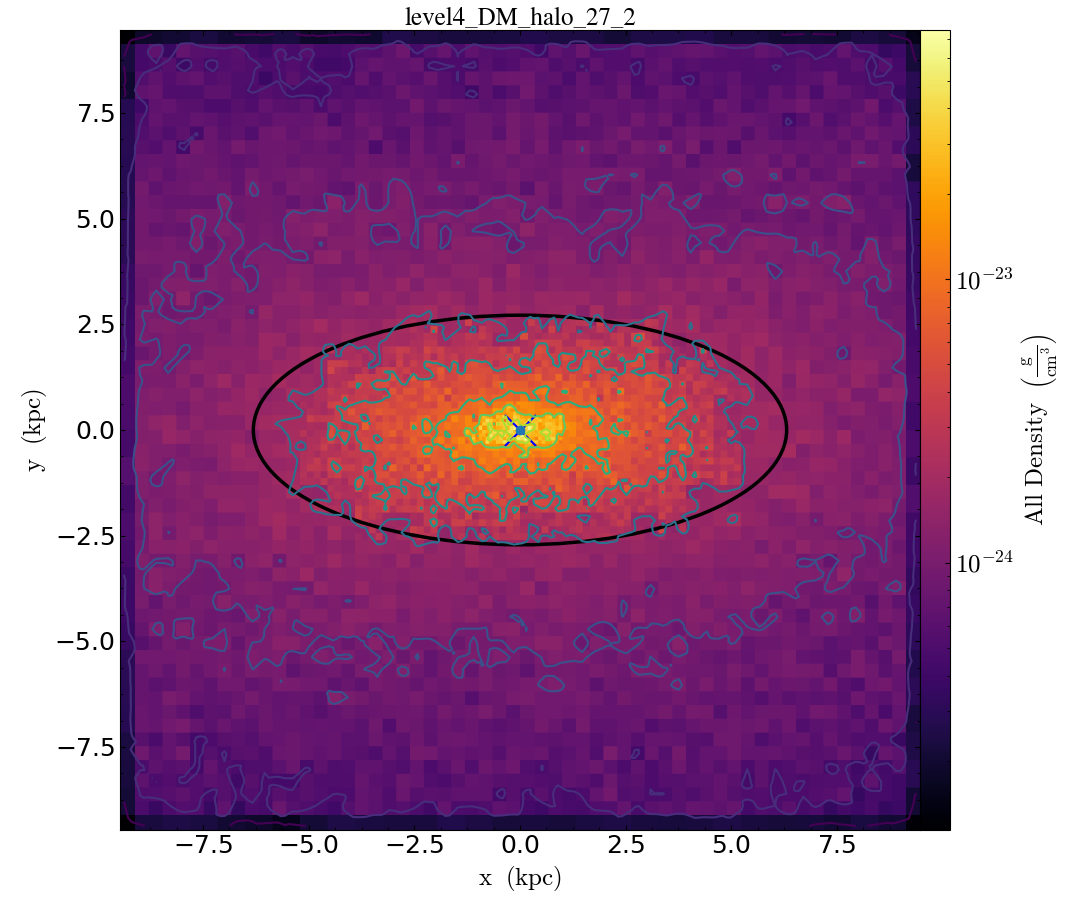
\includegraphics[width=0.5\columnwidth]{./pics/MHD_Vs_DM/level4_DM_halo_27_inner.png}}
  \hfill
  \subfloat[halo 27 DM shape at big radius]{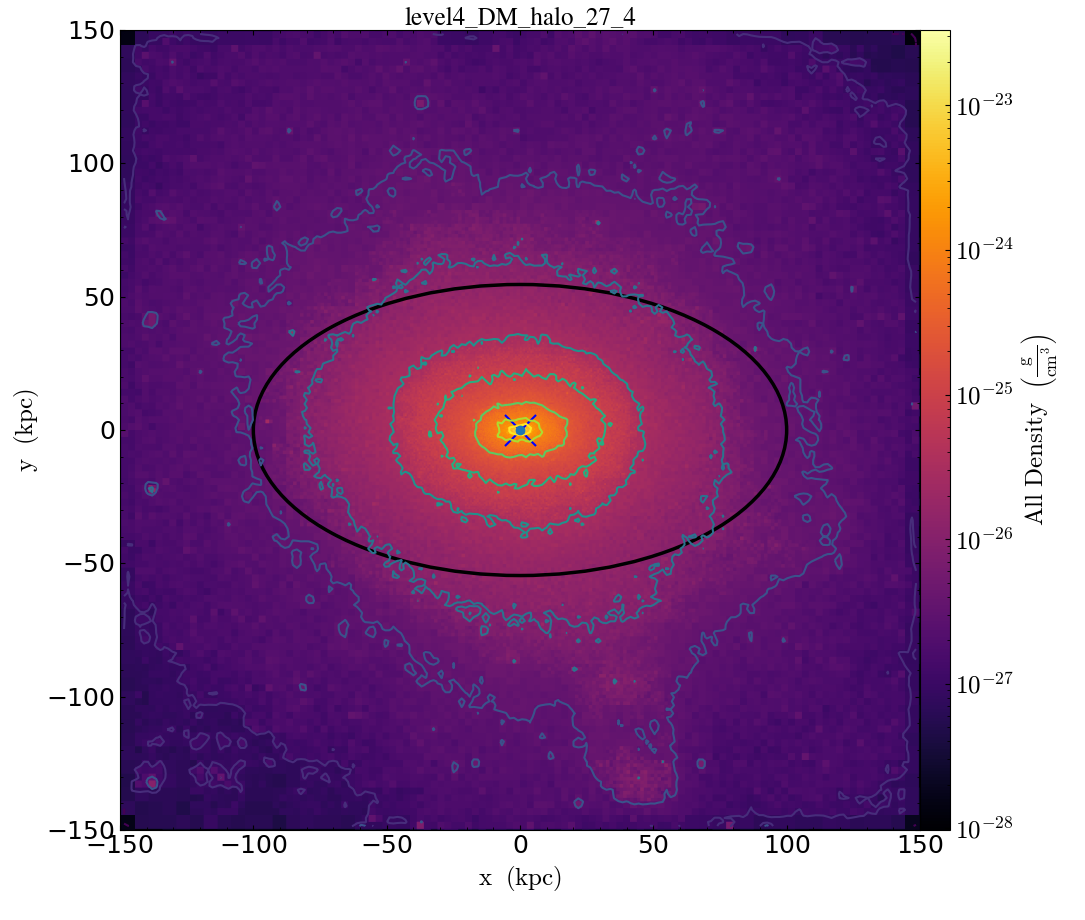
\includegraphics[width=0.5\columnwidth]{./pics/MHD_Vs_DM/level4_DM_halo_27_outter.png}}
  \hfill
  \caption{DM density for inner (outer) parts of the halo 27 on the left (right) part. The horizontal (vertical) axes are aligned to the major (medium) axes. (optimaze space and description) }
  \label{fig:slices}
\end{figure}

We found that most halos exhibit a monotonically-increasing somewhat steady tendency of its axial ratios $b/a,c/a$  with radius, which is well exemplified on figure \ref{fig:DM_MHD}. There are some special cases in which fluctuations of the local DM density field affects this relation, but in average, this monotonic and steady tendency is clear and can be consulted on table \ref{table:DM table}. To ilustrate the average behavior, as well as some peculiarities, we resume the results of the 30 auriga simulations on the figure \ref{fig:Triax_DM} where each shape represents a point in the triaxiality plane $c/a$ Vs $b/a$. Check Vera-ciro onthis.\\

\begin{figure}
\centering
{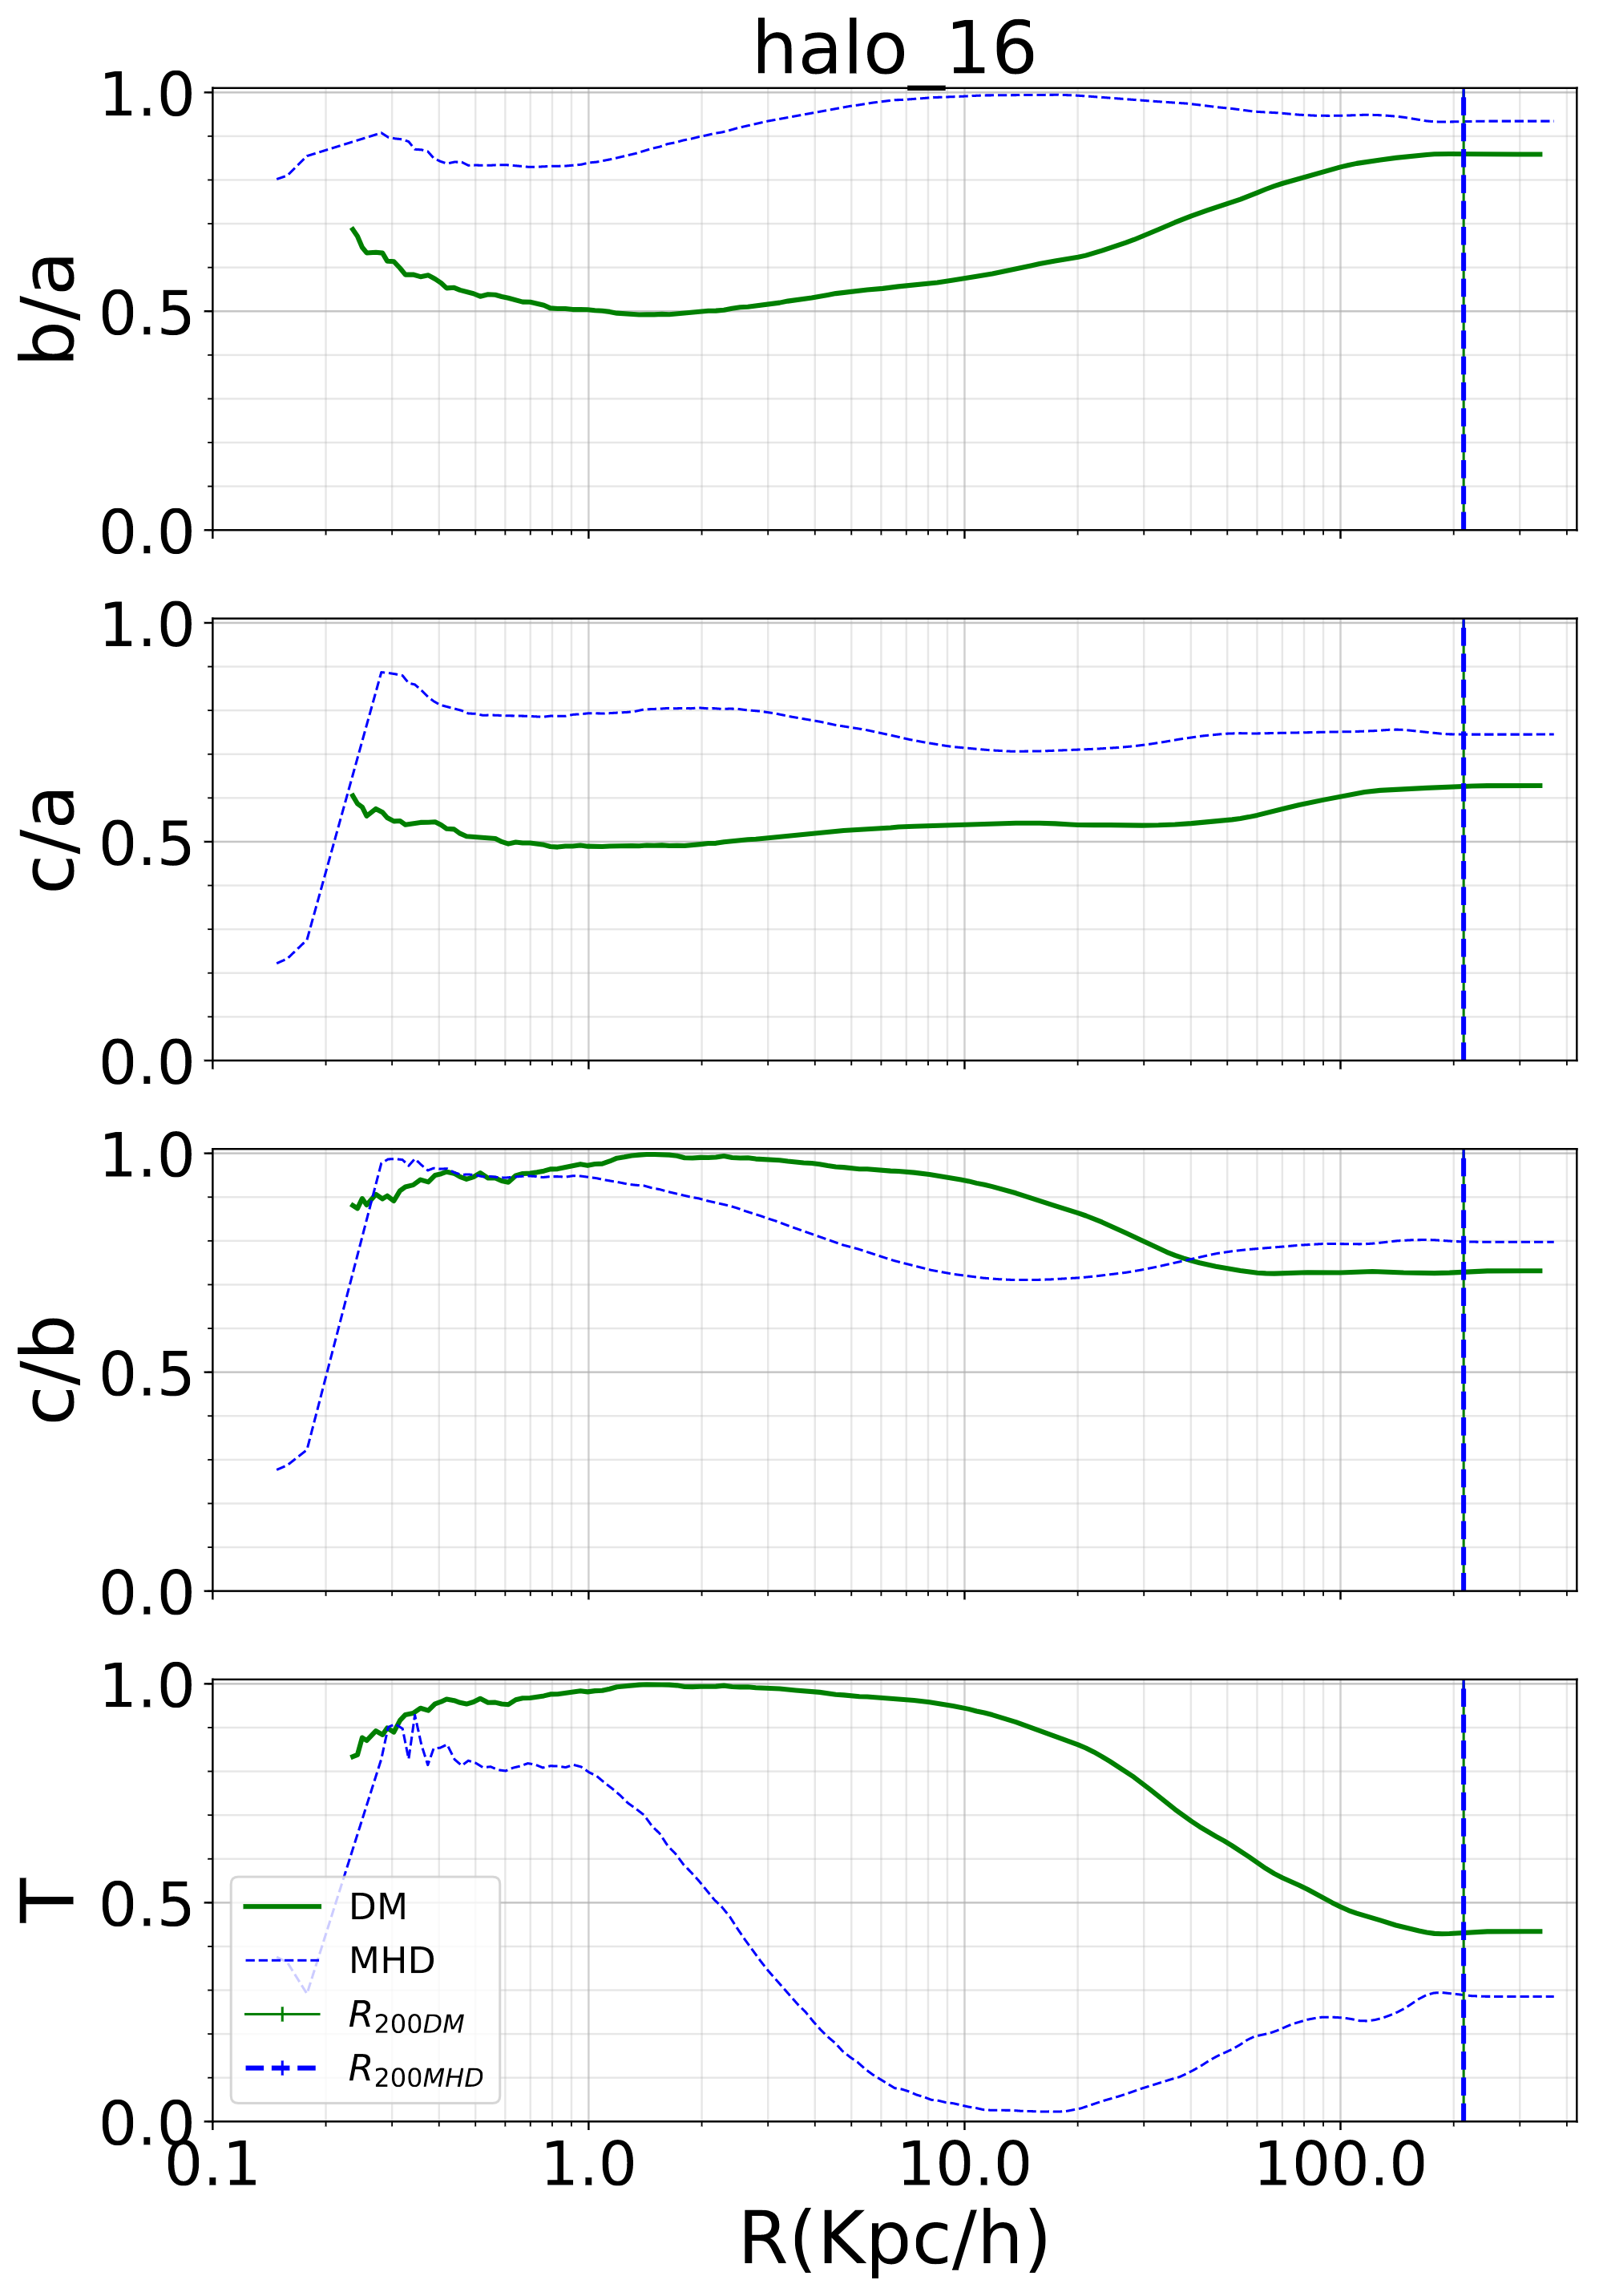
\includegraphics[width=0.8\columnwidth]{./pics/halo16.png}}
\caption{Radial profile for axial ratios and the triaxiality parameter $T=\frac{1-b/a}{1-c/a}$ for halo 16.}
\label{fig:DM_MHD}
\end{figure} 

 
\begin{figure}
  \centering
 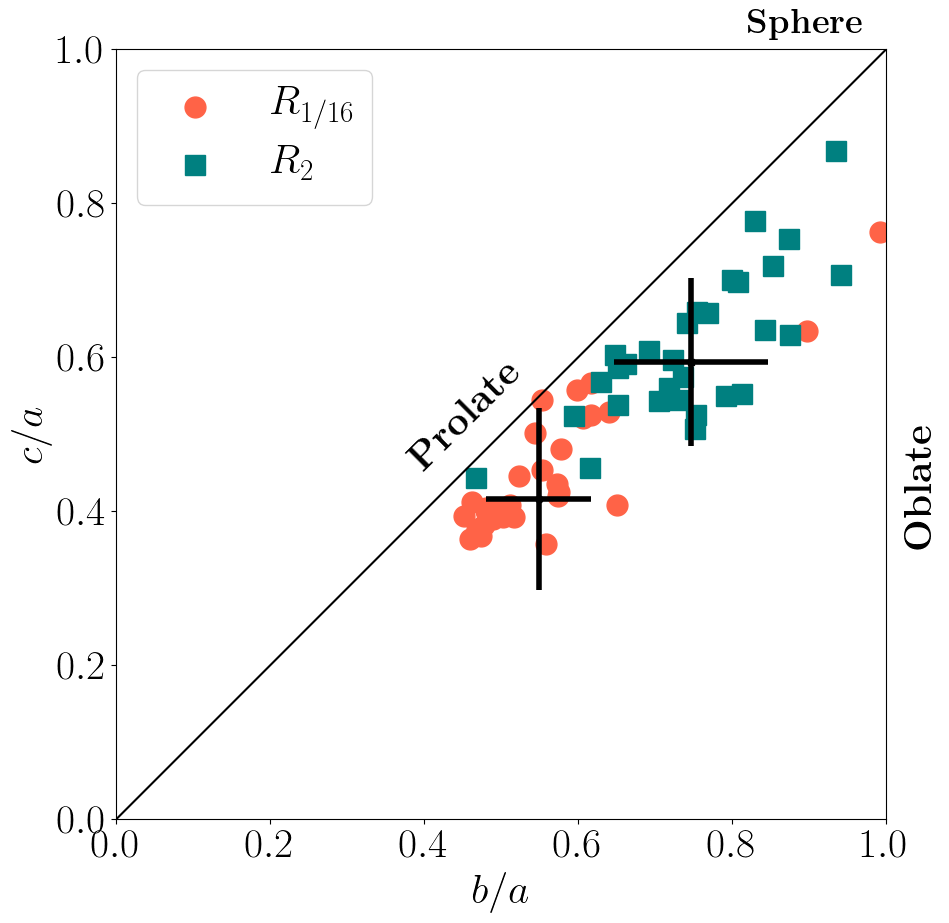
\includegraphics[width=0.9\columnwidth]{./pics/Triaxial_Plane/Triax_DM.png}
  
  \hfill
  \caption{Shape of each halo on the plane $c/a$ Vs $b/a$. Errorbar shows median and errors for each sampled radii. }
  \label{fig:Triax_DM}
\end{figure}

\begin{table}
\setlength{\tabcolsep}{3pt}
\begin{tabular}{l|cccccc}
 &$R_{1/16}$& $R_{1/8}$& $R_{1/4}$& $R_{1/2}$& $R_1$ & $R_2$\\
\hline \hline
$\bar{q}$&$0.55^{+0.07}_{-0.07}$&$0.57^{+0.09}_{-0.08}$&$0.61^{+0.15}_{-0.08}$&$0.65^{+0.18}_{-0.10}$&$0.70^{+0.13}_{-0.10}$&$0.75^{+0.10}_{-0.10}$ \\ [0.1cm]
$\bar{s}$&$0.42^{+0.12}_{-0.03}$&$0.45^{+0.11}_{-0.04}$&$0.49^{+0.09}_{-0.05}$&$0.52^{+0.10}_{-0.05}$&$0.56^{+0.10}_{-0.05}$&$0.59^{+0.11}_{-0.06}$ \\ [0.1cm]
$\bar{T}$&$0.89^{+0.03}_{-0.08}$&$0.88^{+0.04}_{-0.12}$&$0.84^{+0.08}_{-0.23}$&$0.81^{+0.08}_{-0.29}$&$0.75^{+0.14}_{-0.25}$&$0.71^{+0.16}_{-0.19}$ \\ [0.1cm]

\hline
\end{tabular}
\caption{Median values of axial ratios $q,s$ and triaxiality parameter $T$ for DM halos in DM-only simulations at different radii (columns). }
\label{tabe:DM table}
\end{table}

Concerning MHD halos, \textit{prescindible?(((the expected tendency is not clear. Some studies claim that the DM halo must be oblate, at least in the vicinities of the disk, to ensure its stability \cite{disk stability}. However,)))} not much is said about its dependence with radius as previous studies focus rather on the effects of baryons on the dynamics of the halo at fixed radii. Examining the representative behaviour of a MHD halo on figure \ref{fig:DM_MHD}, some things are noticeable: first, the DM halo is almost perfectly oblate around $\approx 10-30$Kpc, second, its axial ratio $b/a$ start decreasing very slowly after $50Kpc$ and below $10Kpc$ and third, its axial ratio $c/a$ does not exhibit noticeable change in the whole radial domain. (Pass from representative case to averaged values) These results are statistically supported and sumarized on table \ref{MHD table} and figure \ref{fig:Triax_MHD}\\

\begin{figure}
  \centering
 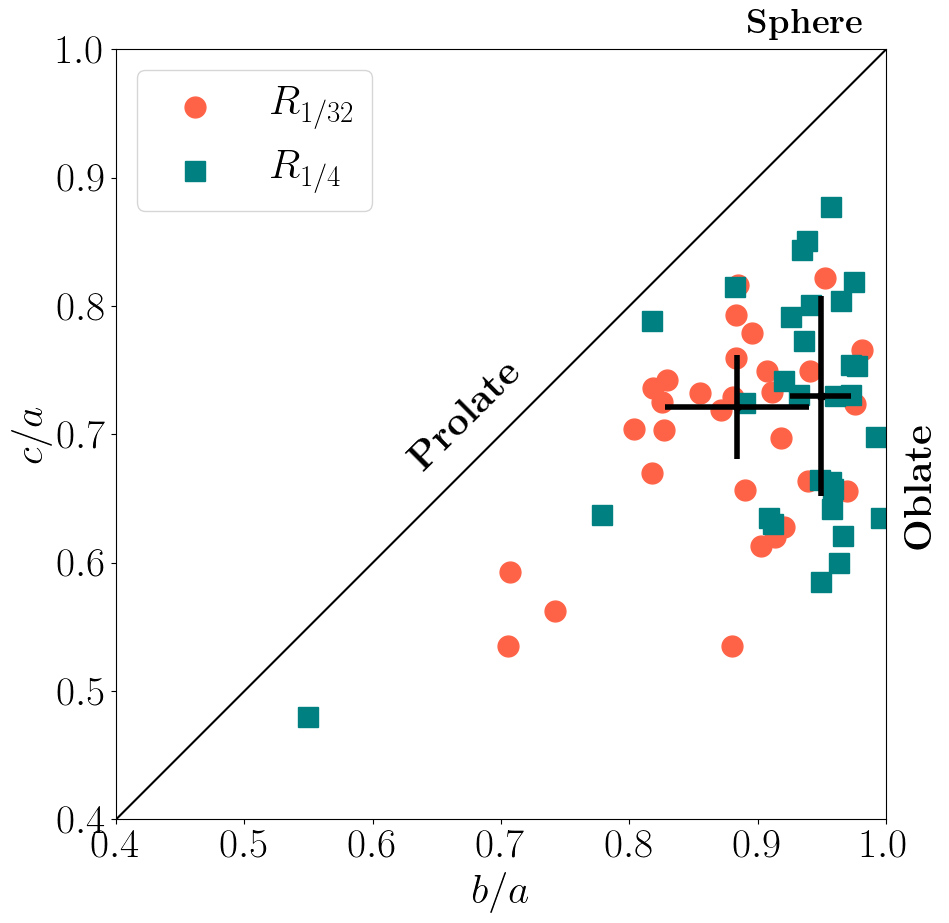
\includegraphics[width=0.9\columnwidth]{./pics/Triaxial_Plane/Triax_MHD.png}
  \hfill
  \caption{Shape of each halo on the plane $c/a$ Vs $b/a$. Errorbar shows median and errors for each sampled radii. }
  \label{fig:Triax_MHD}
\end{figure}


\begin{table}
\setlength{\tabcolsep}{3pt}
\begin{tabular}{l|cccccc}
 &$R_{1/16}$& $R_{1/8}$& $R_{1/4}$& $R_{1/2}$& $R_1$ & $R_2$\\
\hline \hline
$\bar{q}$&$0.93^{+0.04}_{-0.04}$&$0.95^{+0.03}_{-0.03}$&$0.95^{+0.02}_{-0.05}$&$0.93^{+0.04}_{-0.06}$&$0.93^{+0.04}_{-0.10}$&$0.92^{+0.03}_{-0.09}$ \\[0.1cm]
$\bar{s}$&$0.73^{+0.05}_{-0.09}$&$0.73^{+0.07}_{-0.10}$&$0.73^{+0.08}_{-0.10}$&$0.73^{+0.09}_{-0.08}$&$0.75^{+0.07}_{-0.11}$&$0.74^{+0.07}_{-0.10}$ \\[0.1cm]
$\bar{T}$&$0.31^{+0.15}_{-0.22}$&$0.20^{+0.24}_{-0.12}$&$0.24^{+0.20}_{-0.12}$&$0.30^{+0.26}_{-0.16}$&$0.36^{+0.23}_{-0.23}$&$0.39^{+0.26}_{-0.13}$ \\[0.1cm]
\hline
\end{tabular}
\caption{Median values of axial ratios $q,s$ and triaxiality parameter $T$ for DM halos in MHD simulations at different radii (columns). }
\label{tabe:MHD table}
\end{table}

\subsection{Comparison with observational constraints}
To be able to compare our results with observational values, we must relate the calculated quanties with their corresponding isopotential analogue, in which observational constraints are usually presented. For this purpose, we run a simple algorithm to find an approximation of the shape of the isopotential contour. Here, we calculate the mean and standard deviation of the potential over a spherical shell of width equals to $10\%$ of the radius at which it is sampled. Then, we calculate the inertia tensor of particles with potential within $1\sigma$ around the mean potential and calculate its triaxial characterization with the reduced inertia tensor. We repeat the process of calculating the potential mean and standard deviation until convergence is achieved with tolerance of $10^{-4}$. We repeat this process for the different radii from table \ref{tabe:isopotential}. \\

\begin{table}
\setlength{\tabcolsep}{3pt}
\begin{tabular}{l|cccc}
 & $R_{1/8}$& $R_{1/4}$& $R_{1/2}$& $R_1$ \\
\hline \hline
$\bar{q}$&$0.98^{+0.01}_{-0.02}$&$0.97^{+0.01}_{-0.04}$&$0.96^{+0.03}_{-0.06}$&$0.94^{+0.03}_{-0.07}$ \\[0.1cm]
$\bar{s}$&$0.89^{+0.04}_{-0.06}$&$0.88^{+0.04}_{-0.04}$&$0.87^{+0.05}_{-0.05}$&$0.85^{+0.05}_{-0.05}$ \\[0.1cm]
$\bar{T}$&$0.18^{+0.23}_{-0.10}$&$0.36^{+0.19}_{-0.21}$&$0.40^{+0.26}_{-0.20}$&$0.48^{+0.23}_{-0.21}$ \\[0.1cm]
\hline
\end{tabular}
\caption{Median values of isopotential axial ratios $q,s$ and triaxiality parameter $T$ for DM halos in MHD simulations at different radii (columns). }
\label{tabe:isopotential}
\end{table}

As a check of consistency, we compare our new isopotential shape results with the analytic expression of the $(1-q_{\phi})\frac{1}{3}(1-q_{\rho})$ \citep[Binney and Tremaine year]{Binney and tremaine}, taking the volume-enclosed axial ratios as an approximation for the isodensity contour ratios $q_{\rho}$. Although this analytic expression if meant to be used for logarithmic axisymmetric halos, it works well as a first approximation for nearly axisymmetric halos as those produced by our disced galaxies. We find that the difference between the real and the analytic isopotential axial ratios is not bigger than $quantity percent$. With this, we may now present on table \ref{tabe:isopotential} our observationally-comparable results for MHD halos at two important radii one corresponding to the approximate regimes where the MW DM halo is usually constrained.\\   

Little discussion: Are our results congruent with observations? at which radii, does the DM halo shape vary that much?. Which models are favored?\\


\subsection{The rounding effect of baryons}

From the previous characterization of radial shapes it is clear that MHD halos are rounder than DM halos (i.e. axial ratios are bigger) at every sampled radii. This can be compared on tables \ref{tabe:DM table} and \ref{tabe:MHD table} or at the representative example on figure \ref{fig:DM_MHD}. From there, it is also noticeable that the rounding effect of baryons is stronger at the disk regime, where the DM halo is almost perfectly oblate. Furthermore, MHD halos tend towards more oblate shapes (T < 0.5) despite DM halos tendency towards more prolate shapes (T>0.5).\\

This rounding effect is expected from the gravitational effect of the flattened axisymmetric galactic disk. It is also reasonable that this effect is not as strong at $\approx 100$Kpc, where the disk potential is dimmer compared to the DM halo potential. Keeping this in mind, one would expect that the rounding effect of baryons is related to some galactic parameters such as its component masses and radii. However, even for the parameter of highest correlation with this rounding effect (the baryonic fraction), the relation is not clear nor conclusive due to the dispersion from galaxy peculiarities. In figure \ref{fig:Star_Density_effect} we plot the ratios $c/a$ compared to the baryonic fraction of each galaxy. Although some linear tendency is suggested qualitatively, the dispersion of the sample is very high to obtain some conclusive relation. This is an evidence that adiabatic-contraction models are not realistic as they may neglect some effects of the galaxy evolution in the whole cosmological context. \\

\begin{figure}
	% To include a figure from a file named example.*
	% Allowable file formats are eps or ps if compiling using latex
	% or pdf, png, jpg if compiling using pdflatex
	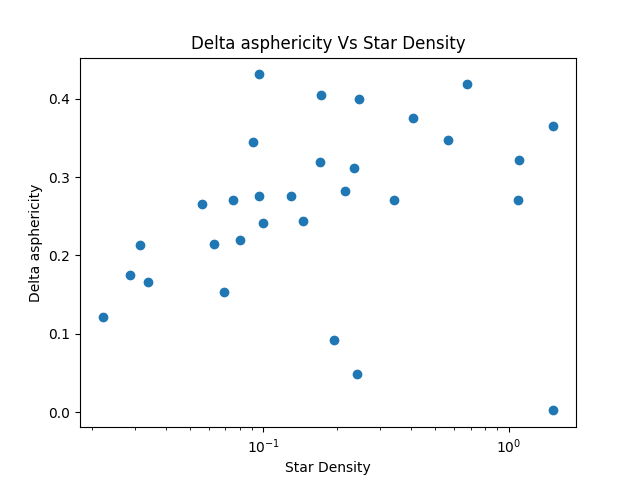
\includegraphics[width=\columnwidth]{./pics/Delta asphericity Vs Star Density.png}
    \caption{Difference in asphericities between MHD and DM shapes Vs Star Density of the simulation.}
    \label{fig:Star_Density_effect}
\end{figure}

\textbf{Actually we have not examined the relation of c/a in MHD halos with some measure of c/a from the disk, that is something like Zdisk/Rdisk. This actually would make more sense from a physical point of view: effect of the potential.}

Although the effect of the baryonic disk on the shape of the DM halo is a reasonable explanation for the rounding effect, it does not actually explain the deviation from oblateness of MHD halos at $r<10$Kpc. In other words, if the disk is perfectly axisymmetric, there must be some source of triaxiality at $r<10$Kpc to explain the low axial ratios.\\   

\textit{ Talk about source of triaxiality at the inner parts of the halos (bar?). This source of triaxiality at the inner parts explains why the axial ratios are $\approx 0.95$ and not exactly $1$. We should also discuss that the decrease in the axial ratios for bigger radii may actually be bigger/steeper but it is dimmed by the contribution of inner parts.}\\
%
%\begin{figure}
%  \centering
%  \subfloat[Level4 MHD Vs DM at inner regions]{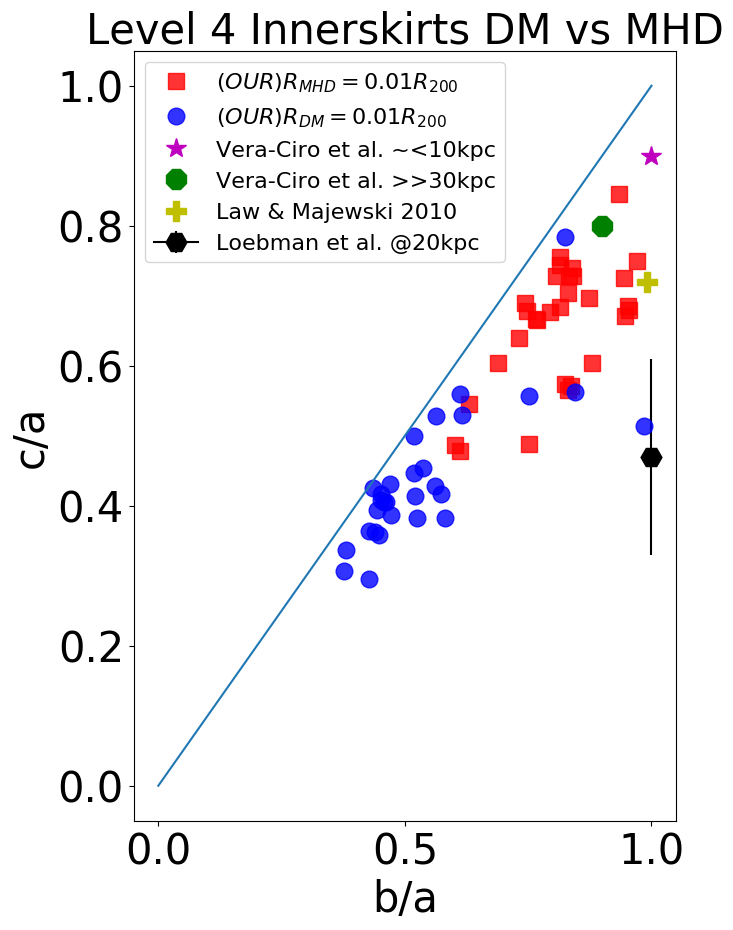
\includegraphics[width=0.5\columnwidth]{./pics/Triaxial_Plane/Triaxiality_Inner_lvl4.png}}
%  \hfill
%  \subfloat[Level4 MHD Vs DM at outer regions]{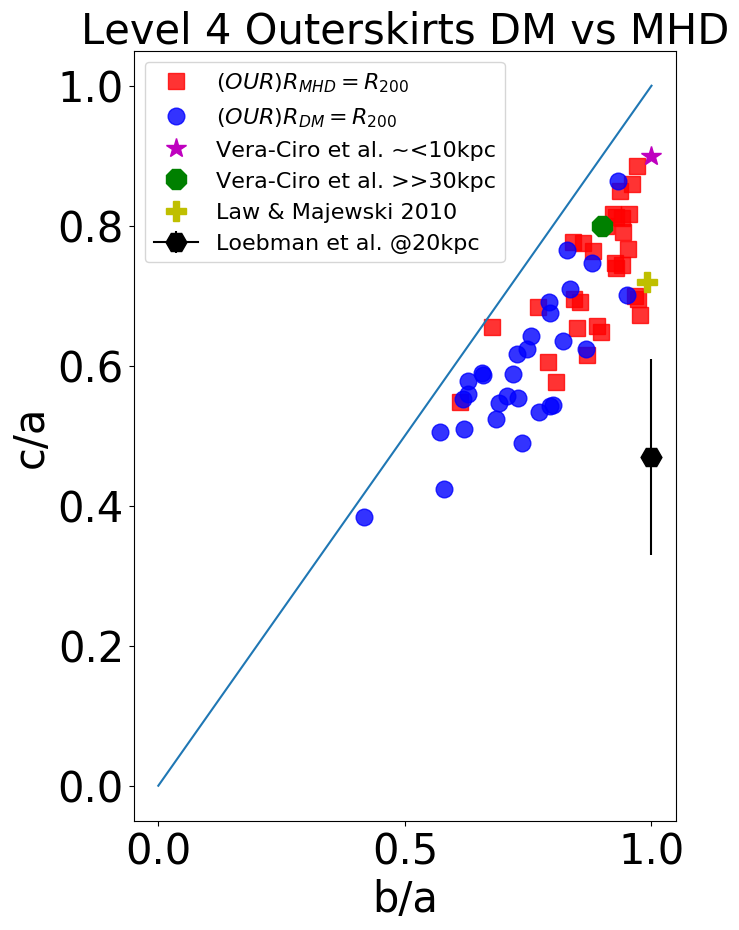
\includegraphics[width=0.5\columnwidth]{./pics/Triaxial_Plane/Triaxiality_Outter_lvl4.png}}
%  \hfill
%  \caption{Axial ratios as shown on $c/a$ Vs $b/a$. Each dot represents a halo shape at some radius. Some observational constraints are plotted alongside our results. Here, dots are clustered, proving the general tendence of halos to get rounder on the outer parts.(Optimize space. caption replaces title.  Present constraints representation of density)}
%  \label{fig:Triaxiality_Inner_Outer}
%\end{figure}


\subsection{The historical shape}
One of the principal motivations to study the radial dependence of the DM halo shape is that it may encode some clues about its formation history. We have already shown that DM-only halos seem to exhibit a steady and monotonous growth in its axial ratios when sampled at bigger radii. One similar effect can be found if we sample the shape at the virial radius, this time at varying redshift. It is easy to see that the axial ratios increase with decreasing redshift, which is expected by the continuous influence of the gravitational potential \cite{VeraCiro}. In figure \ref{fig:RedshiftGood} we present a representative example. \\  
 
\begin{figure}
  \centering
  \subfloat[halo 16 DM]{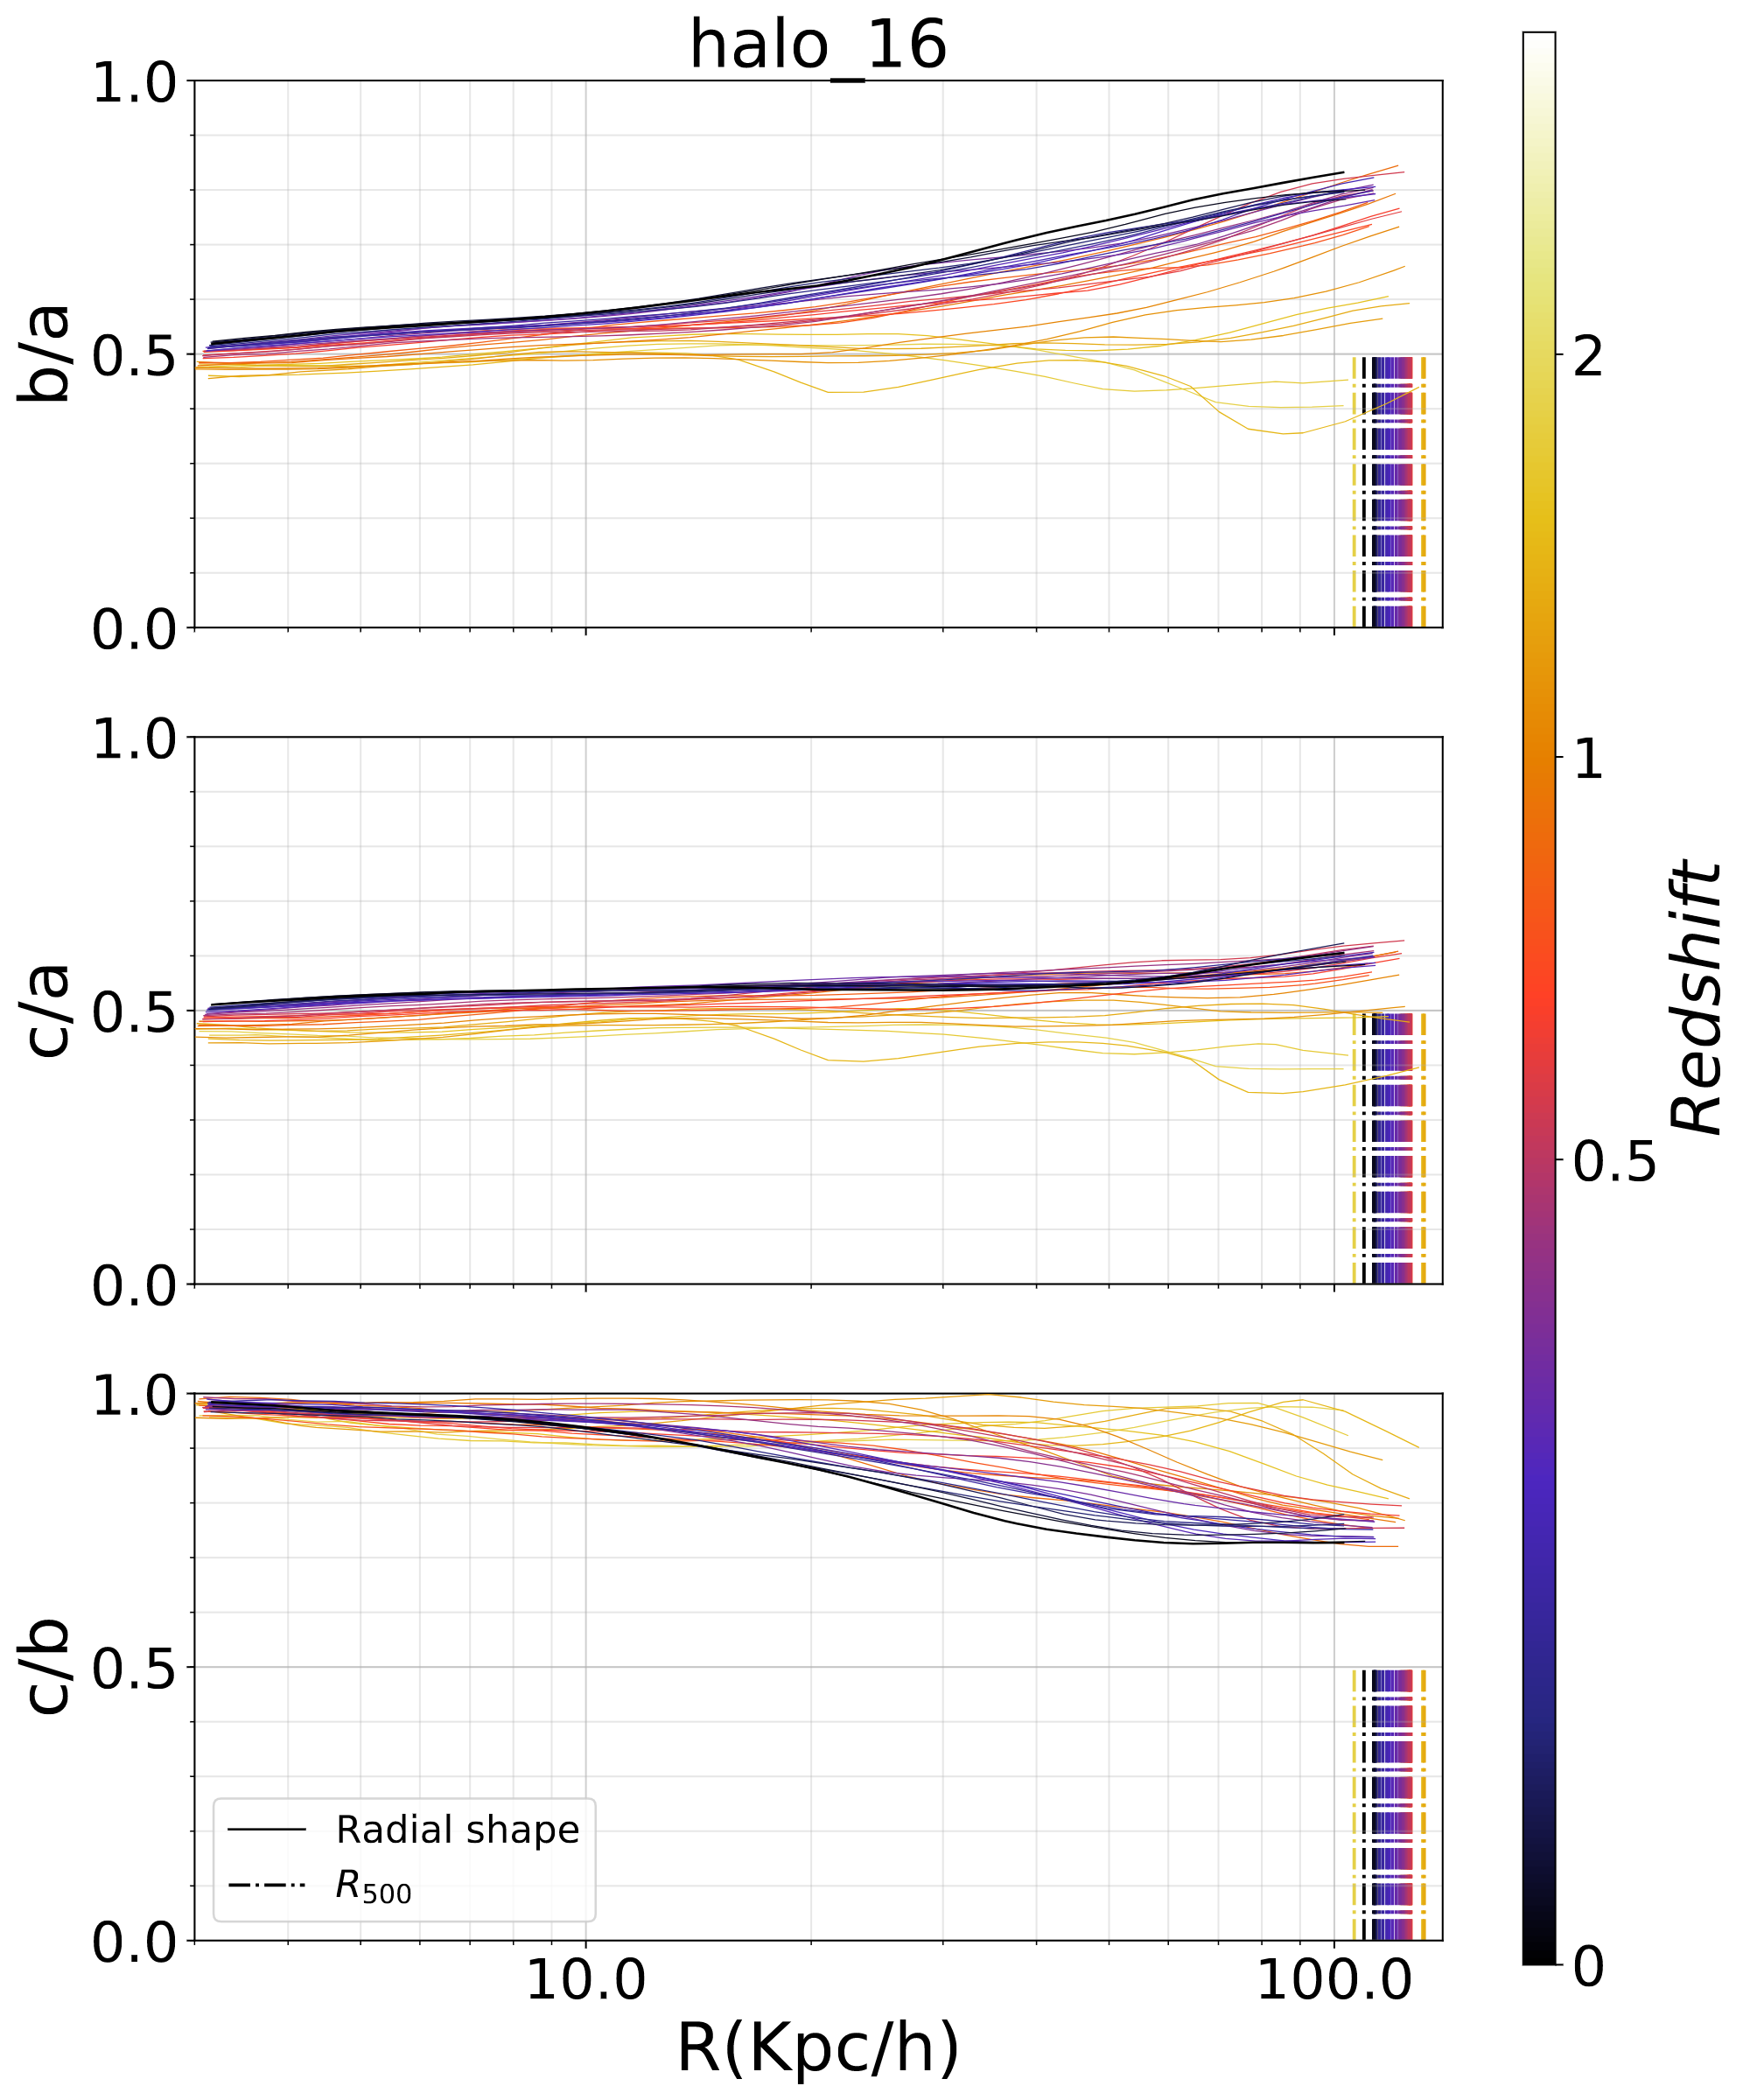
\includegraphics[width=0.5\columnwidth]{./pics/Redshift/halo_16_level3_DM_Z.png}}
  \hfill
  \subfloat[halo 16 MHD]{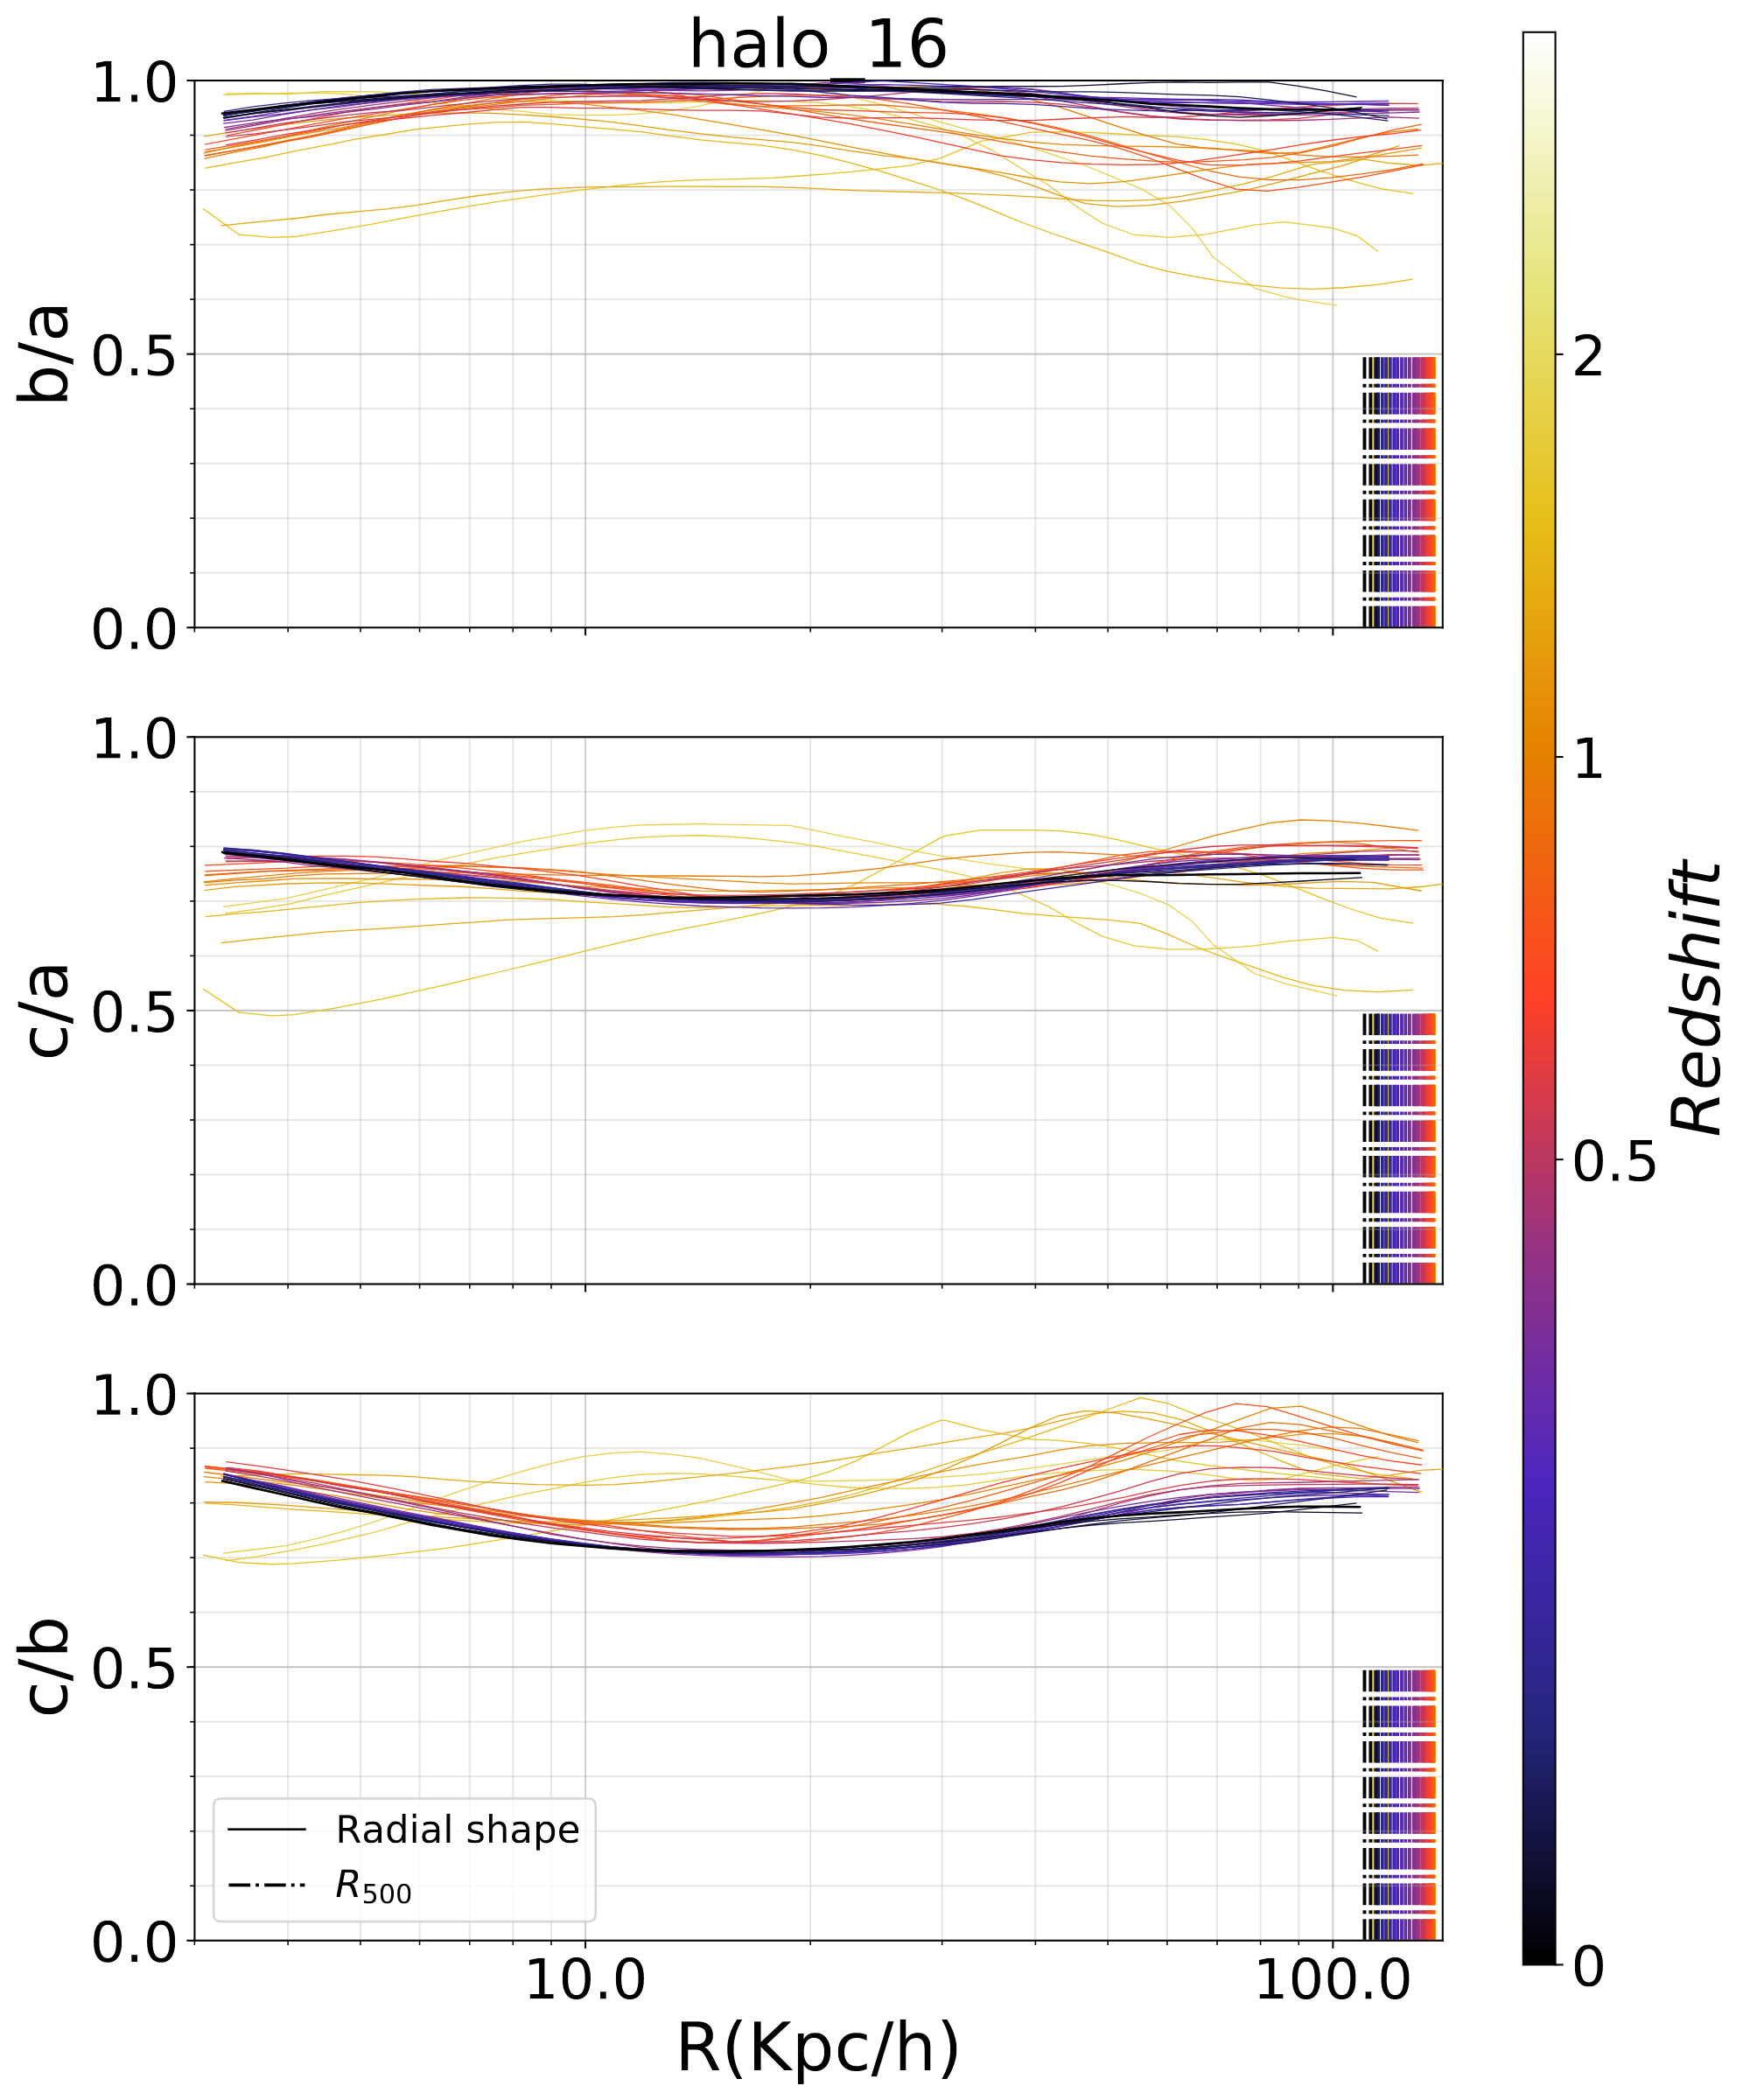
\includegraphics[width=0.5\columnwidth]{./pics/Redshift/halo_16_level3_MHD_Z.png}}
  \caption{Radial profile (comoving) of axial ratios for halo 16 in terms of redshift (color). This halo maintains its shape until $z\approx 1$ obviating the systematic rounding effect in time from asymmetric potentials. }
  \label{fig:RedshiftGood}
\end{figure}


Interestingly, these two parametic plots i.e. $(b/a,c/a)(z=0,r)$ and $(b/a,c/a)(z,r=R_{vir})$ are very correlated for DM-only halos \ref{fig:DM Z Triax}. This means that, for DM-only halos, one can approximate its shape at higher redshift by simply sampling its current shape at a smaller radius \textbf{wording}. This relationship relies strongly on the steady and monotonous tendency of DM halos towards sphericity for bigger radii and smaller redshift.\\


\begin{figure}
	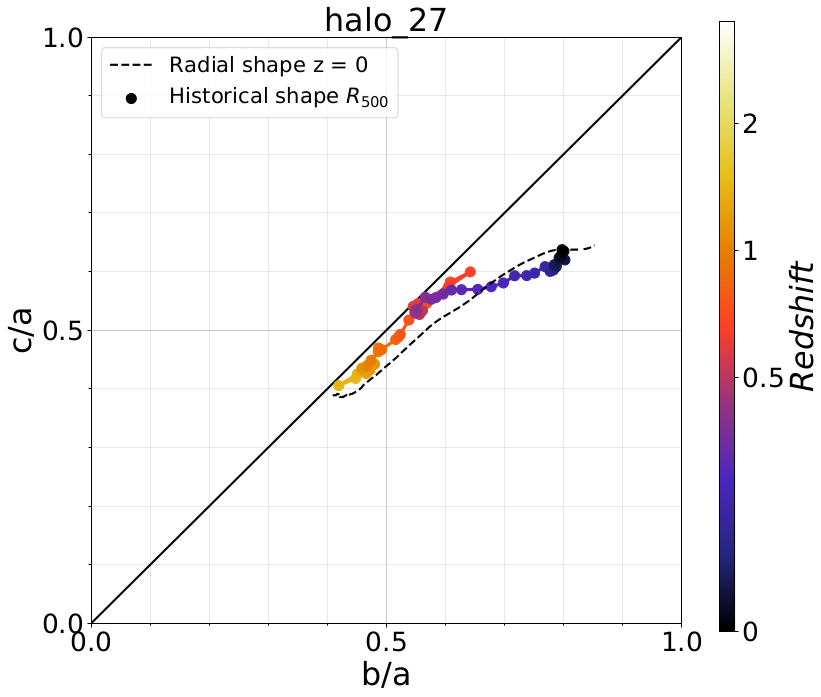
\includegraphics[width=\columnwidth]{./pics/Redshift/halo_27_DM_Z_correlation.png}
    \caption{Difference in asphericities between MHD and DM shapes Vs Star Density of the simulation.}
    \label{fig:DM Z Triax}
    
\end{figure}

MHD halos, on the other hand, do not exhibit tendency towards sphericity with bigger radii, but they do get sistematically rounder at lower redshift as seen in figure \ref{fig:RedshiftGood}. This effectively vanishes this correlation as seen from a DM halo \ref{fig:MHD Z Triax}.\\

\begin{figure}
	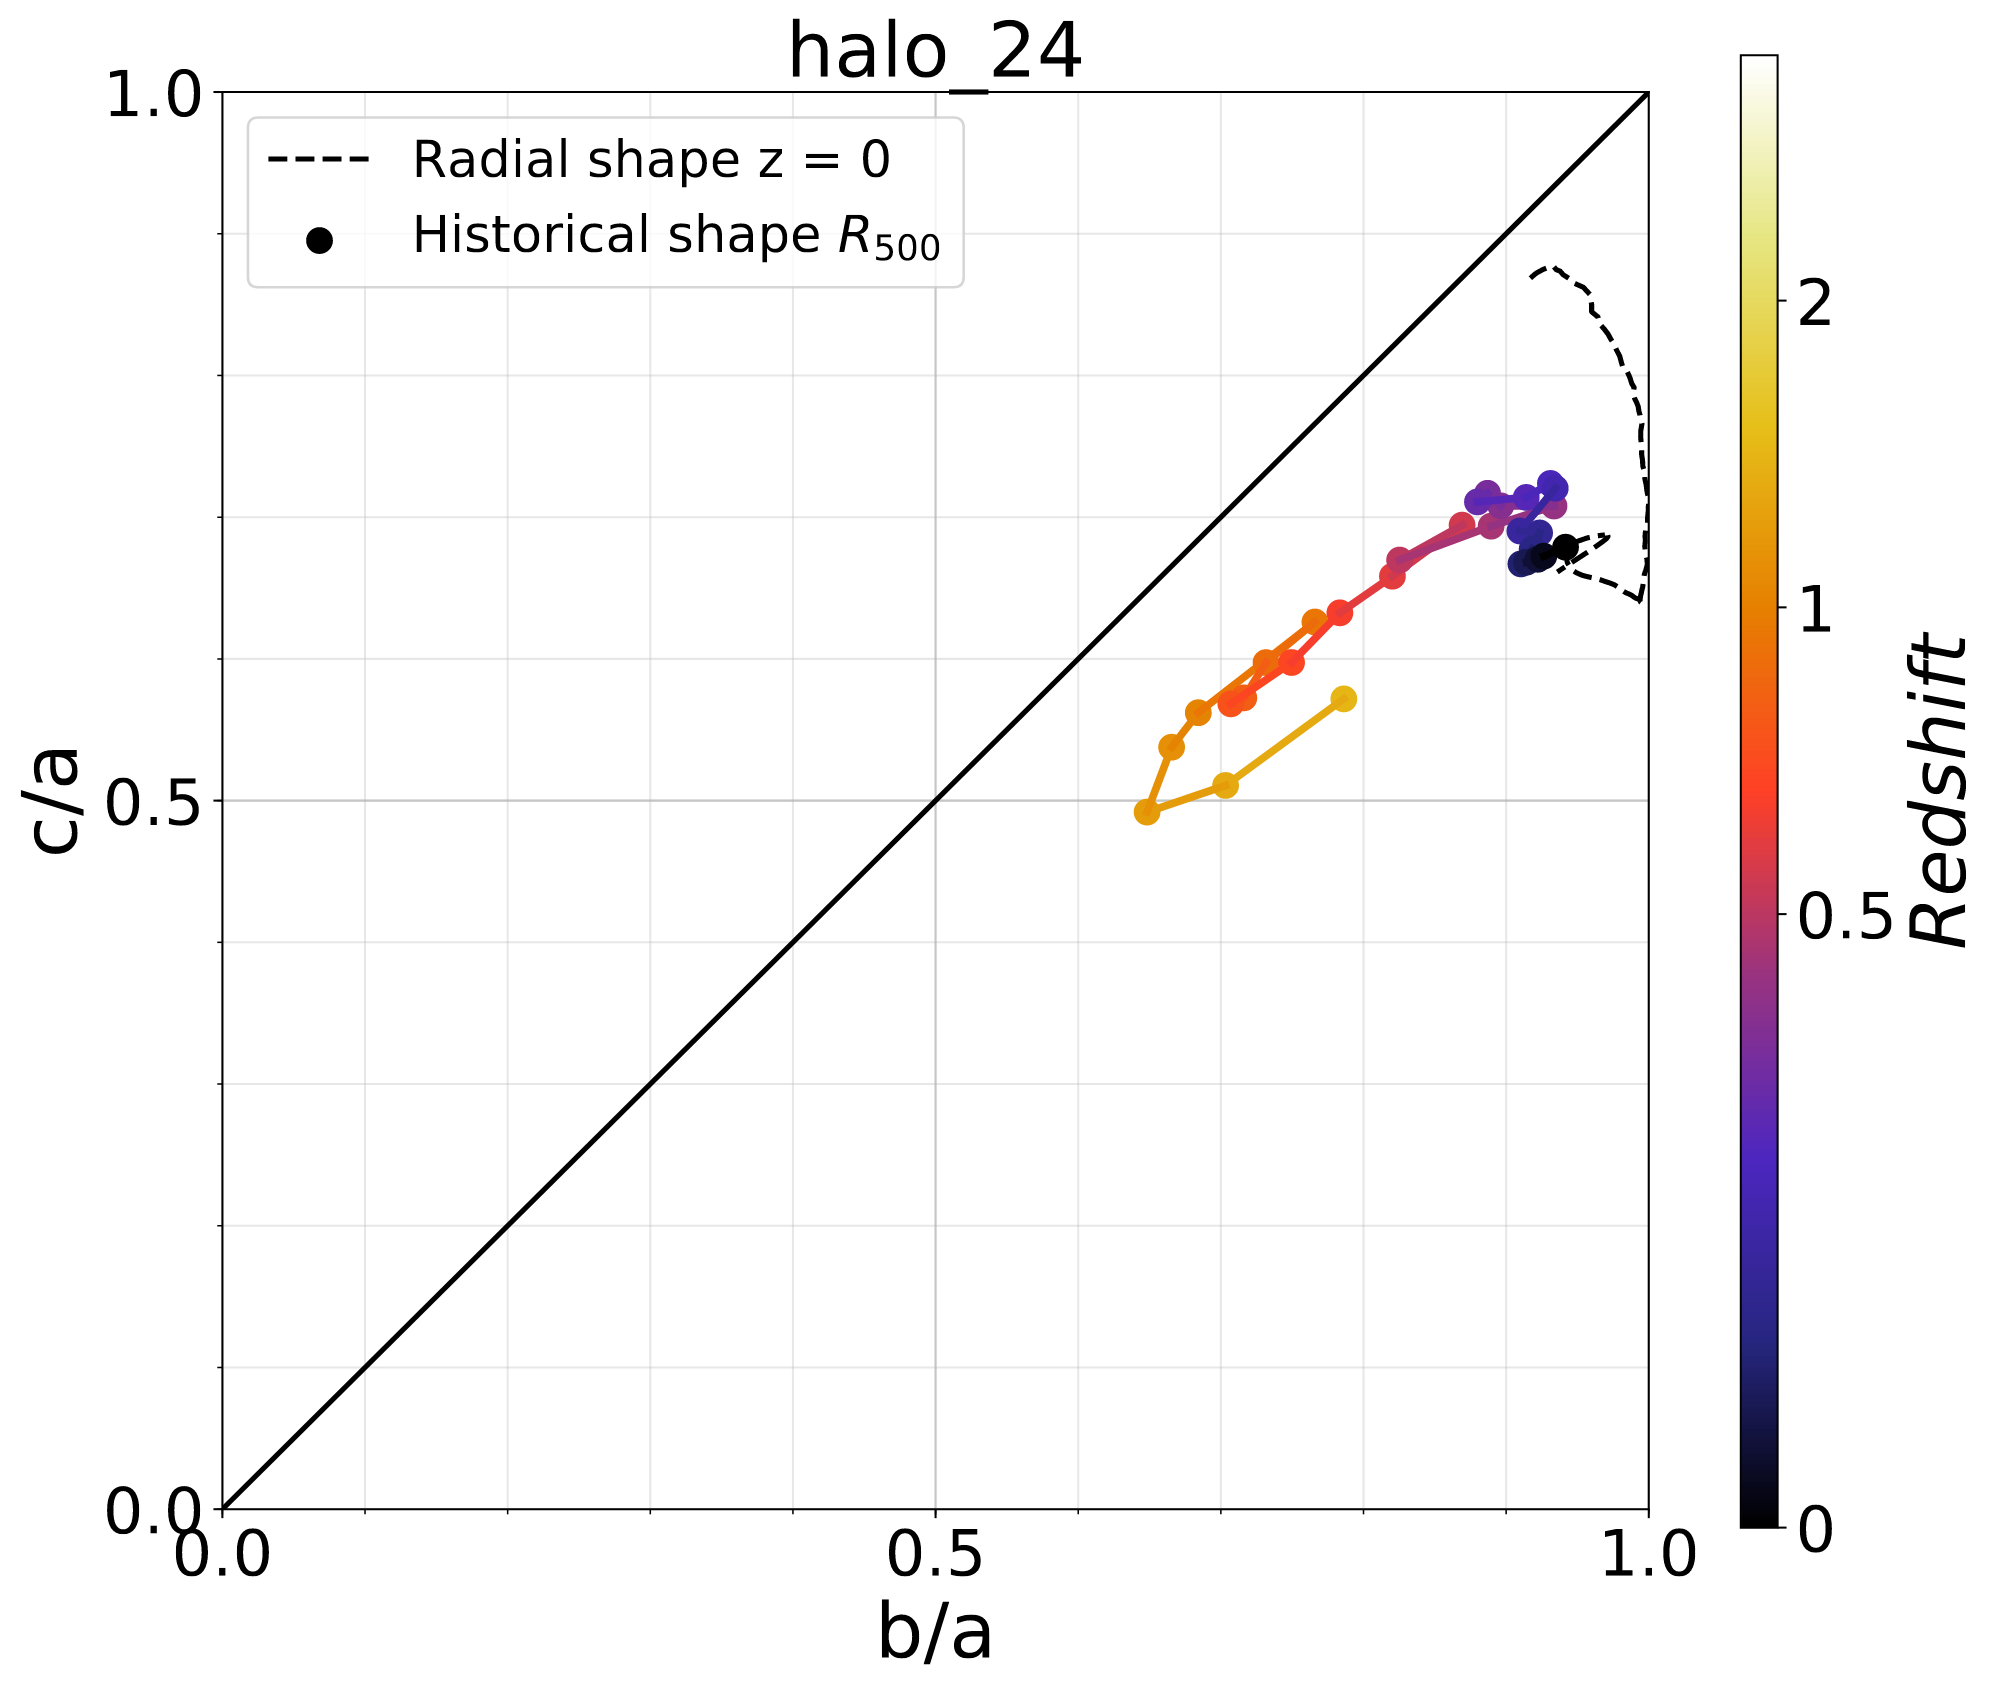
\includegraphics[width=\columnwidth]{./pics/Redshift/halo_24_level3_MHD_Z_Triax.png}
    \caption{Difference in asphericities between MHD and DM shapes Vs Star Density of the simulation.}
    \label{fig:MHD Z Triax}
    
\end{figure}

Better graphics.

%Discuss if this correlation may be recovered if compared for example at Disk radius in stead of virial radius.\\


\subsection{The orientation of the principa axes}

One of the principal assumptions of observational models of the MW's DM halo is that its minor axis is perfectly aligned with the disk axis. Although this is a reasonable assumption to guarantee the stability of the galactic disk in simplified models of isolated galaxies, it may not be the case for galaxies evolved in the whole cosmological context nor at every radii at which the shape is sampled.\\

Therefore, it is of special interest to us to examin the strength of this alignment assumption in the context of simulations. For this purpose, we sampled the shape at 5 different radii and plotted the axial directions, as well as the disk direction in the \textbf{name} diagrams \cite{} (explain diagrams). Explain disk direction calculation.\\

We found that there is not a representative example of what happens in terms of alignments. We found that the majority of the disks are aligned with the minor axis of their DM halo within $\approx 30^o$; in some special cases, this alignment was almost perfect and in some other cases, the DM halo minor axis changed substantially to be able to determine an alignment. In figure \ref{fig:alignment} we present these three cases. \textbf{occurrencies for each case?}


\textit{This is an important result of our study. We study the radial evolution of the principal axes, compared also to the angular momentum vector from the disk. We found that while the angular momentum tend to be aligned with the minor axis of the ellipsoid, this may not be the case all times. When there is an alignment it is usually within 20 degrees (get a histogram of this. and an evolution of this histogram with time). When there is not an alignment, then there is no simple way to determine towards which axis it is oriented. Furthermore, the principal axes alignment usually change with radius (rotation, swap, verify). This ask for relaxation on the strong constrains on the MW DM halo models.}


\begin{figure}
  \centering
  \subfloat[Perfectly aligned Axes]{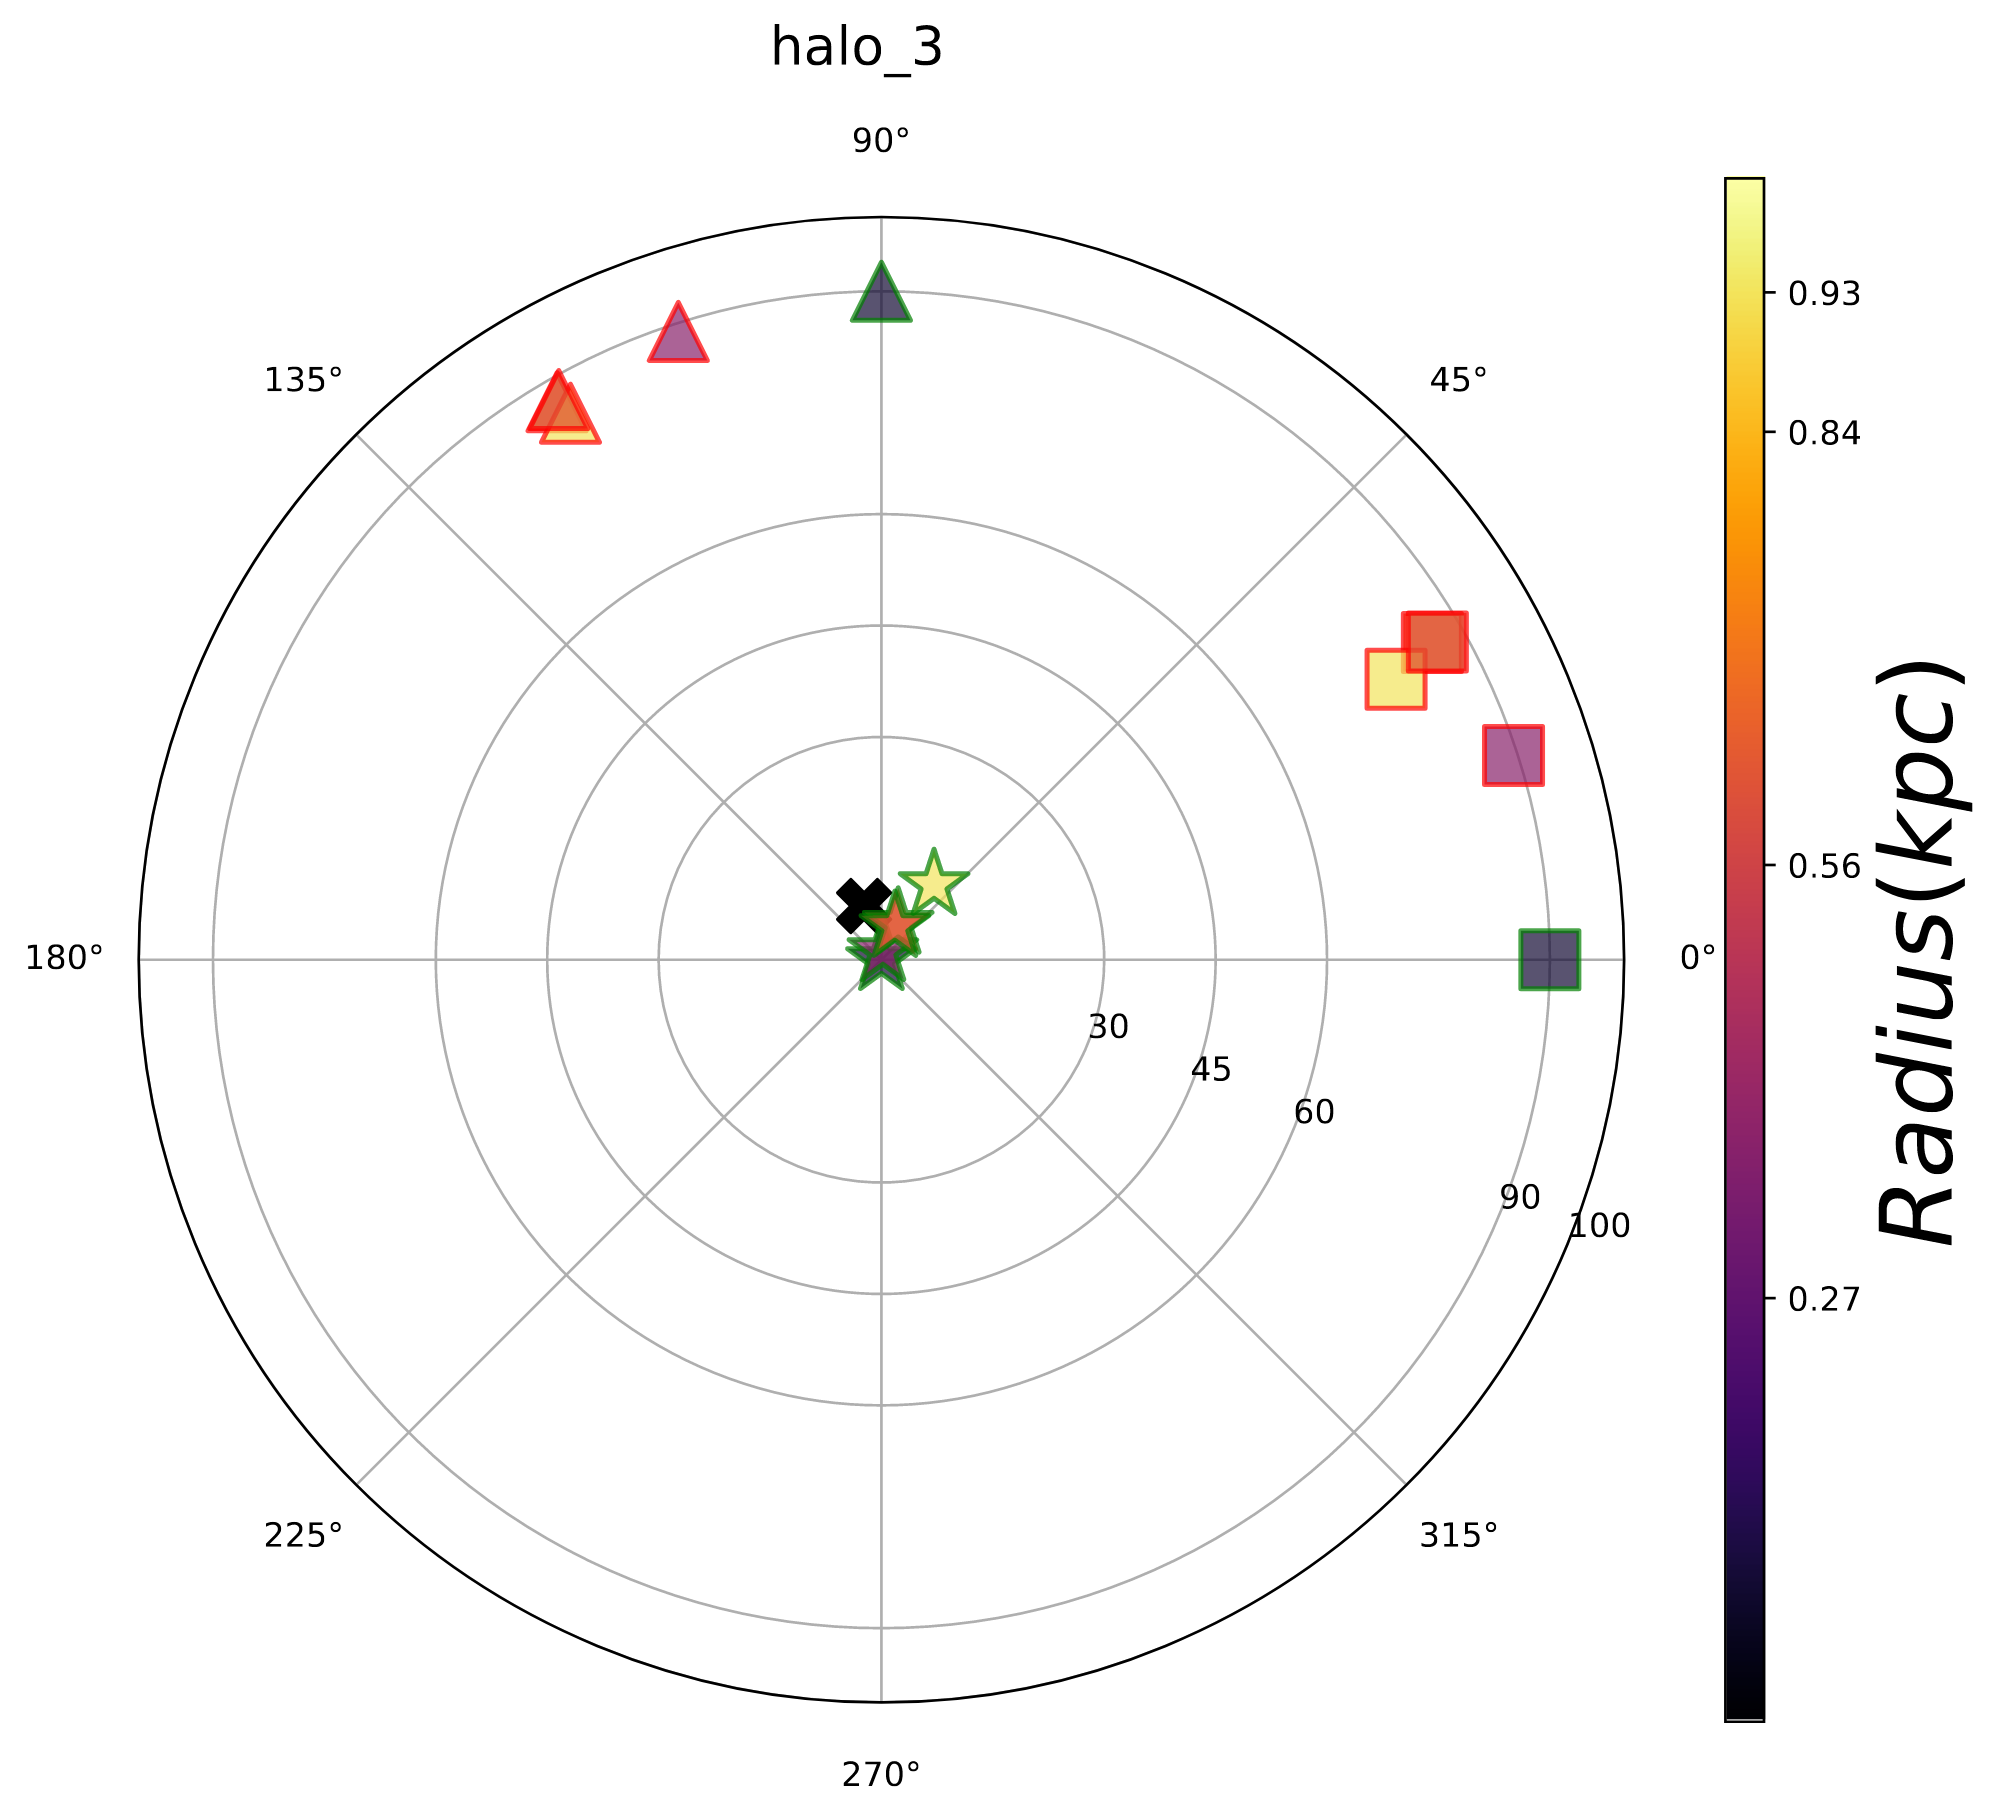
\includegraphics[width=1\columnwidth]{./pics/well_axes.png}}
  \hfill
  \subfloat[Somewhat aligned Axes]{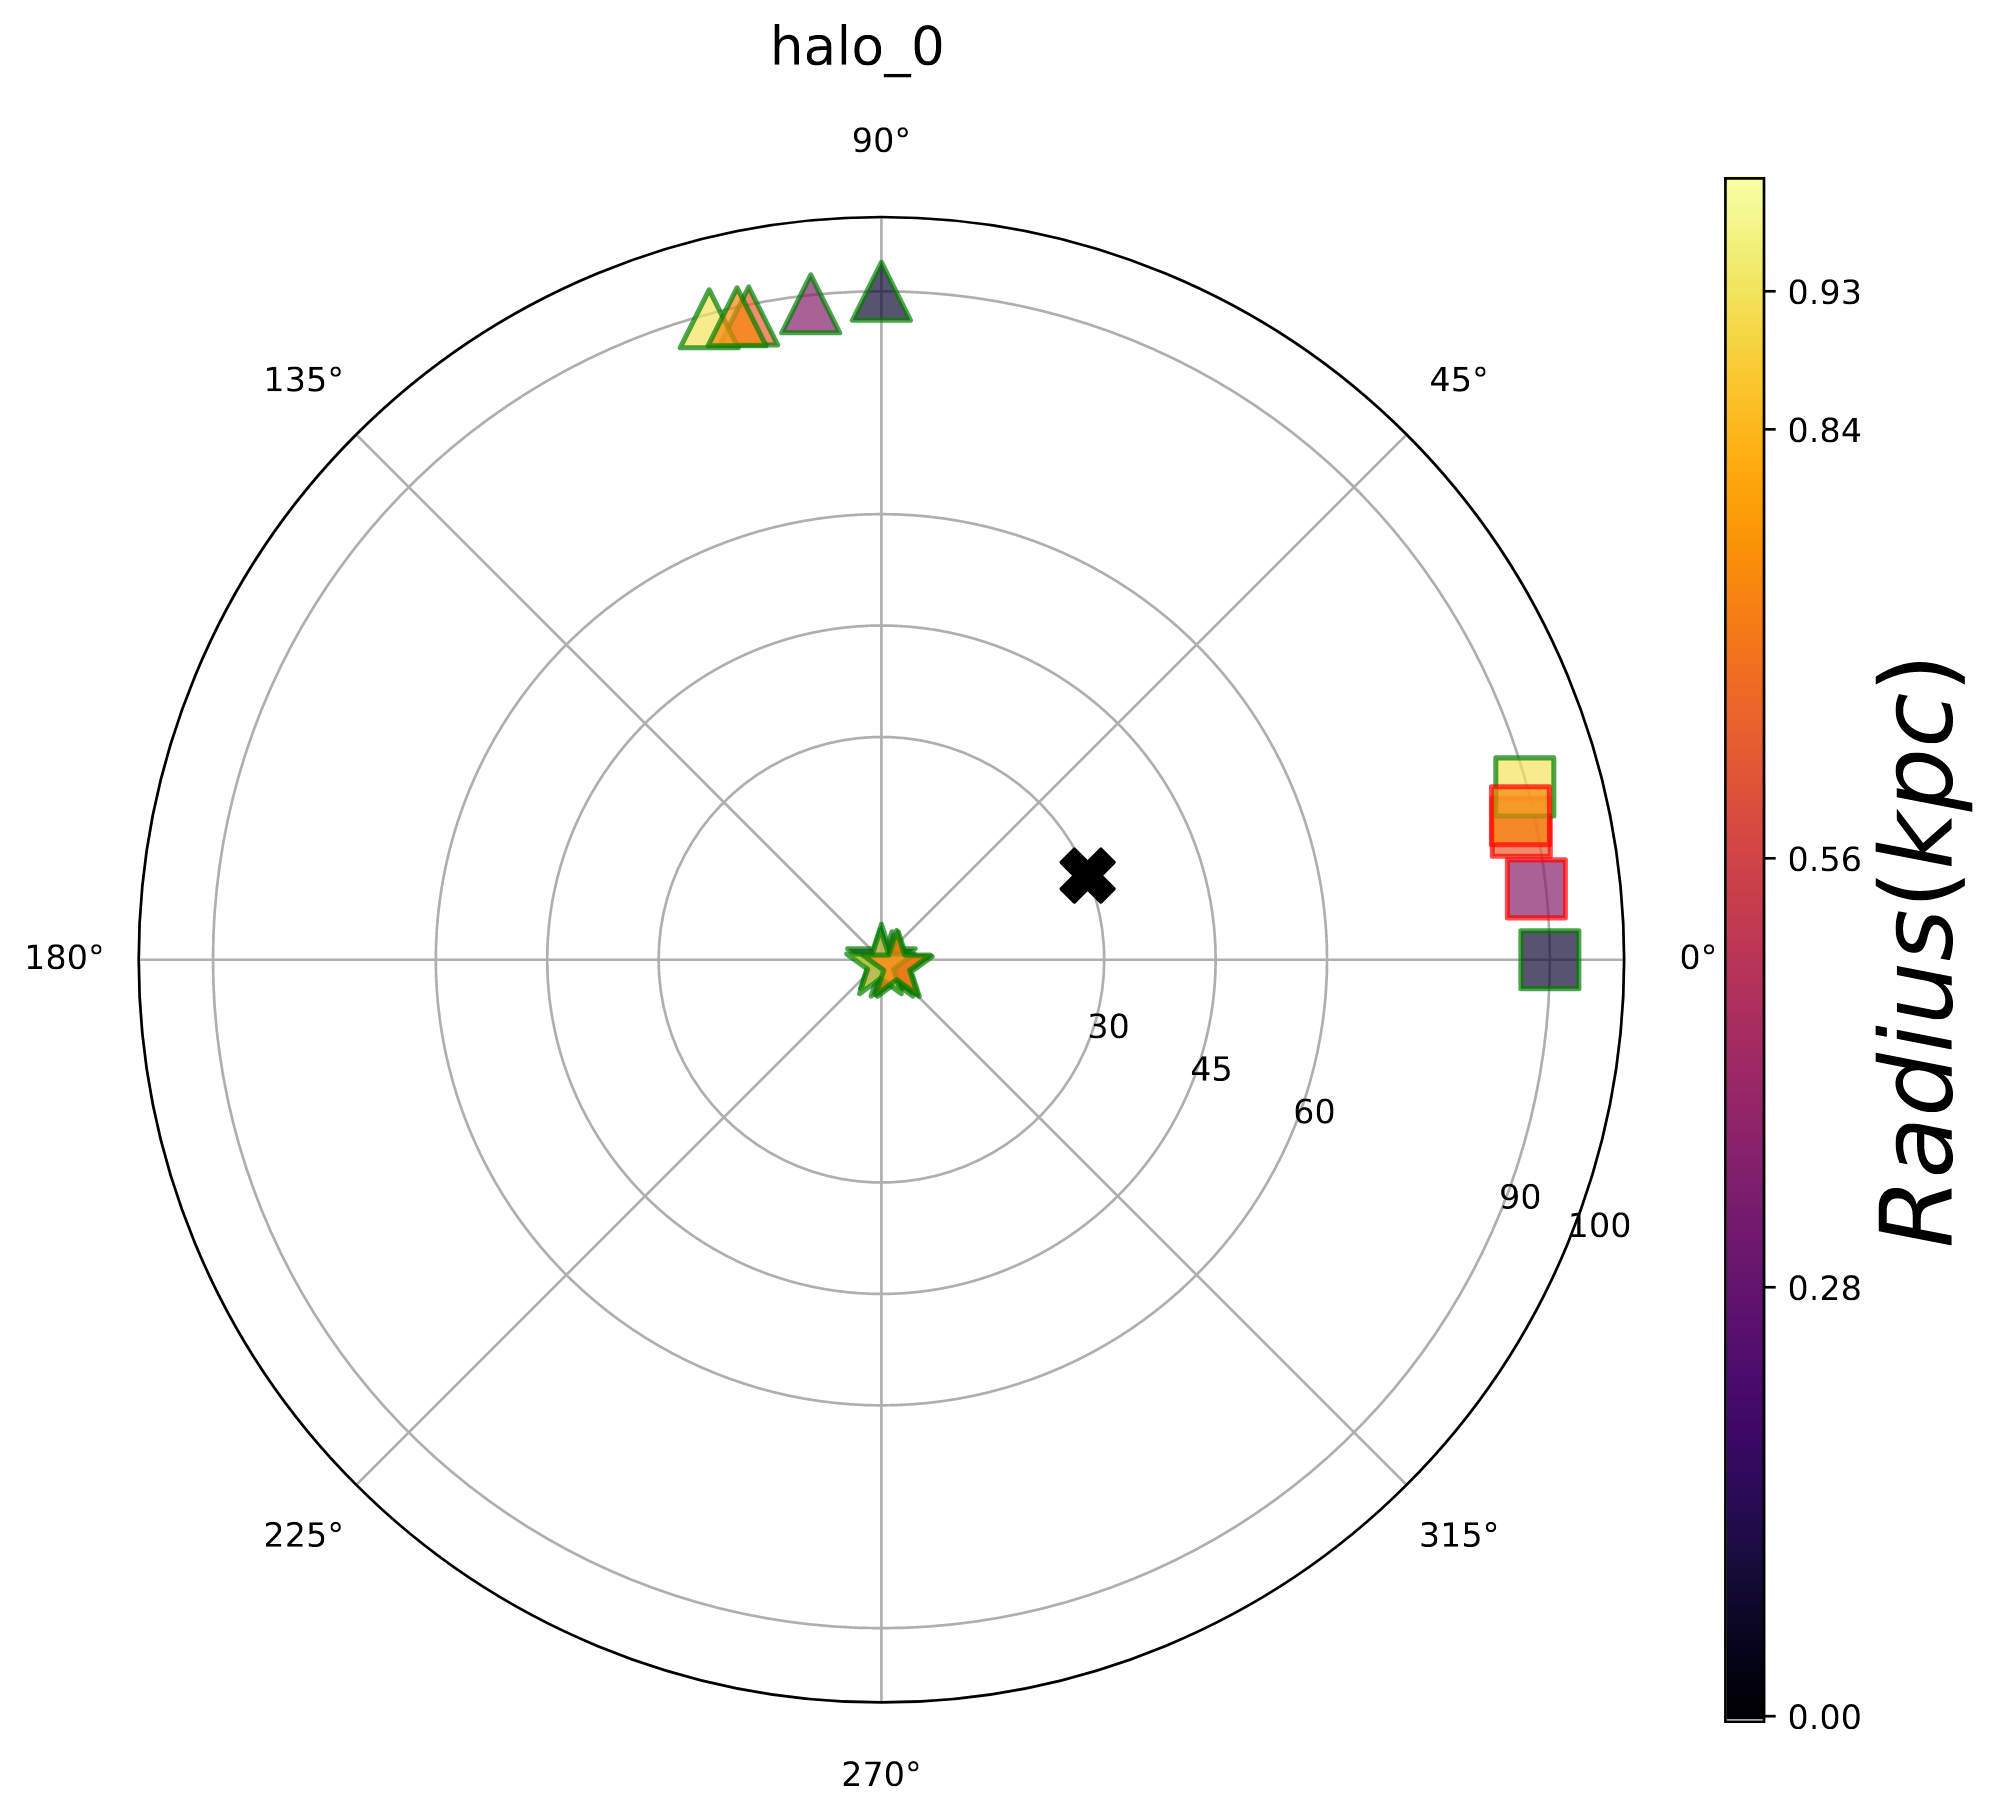
\includegraphics[width=1\columnwidth]{./pics/rotating_axes.png}}
  \hfill
  \subfloat[Chaotic Axes]{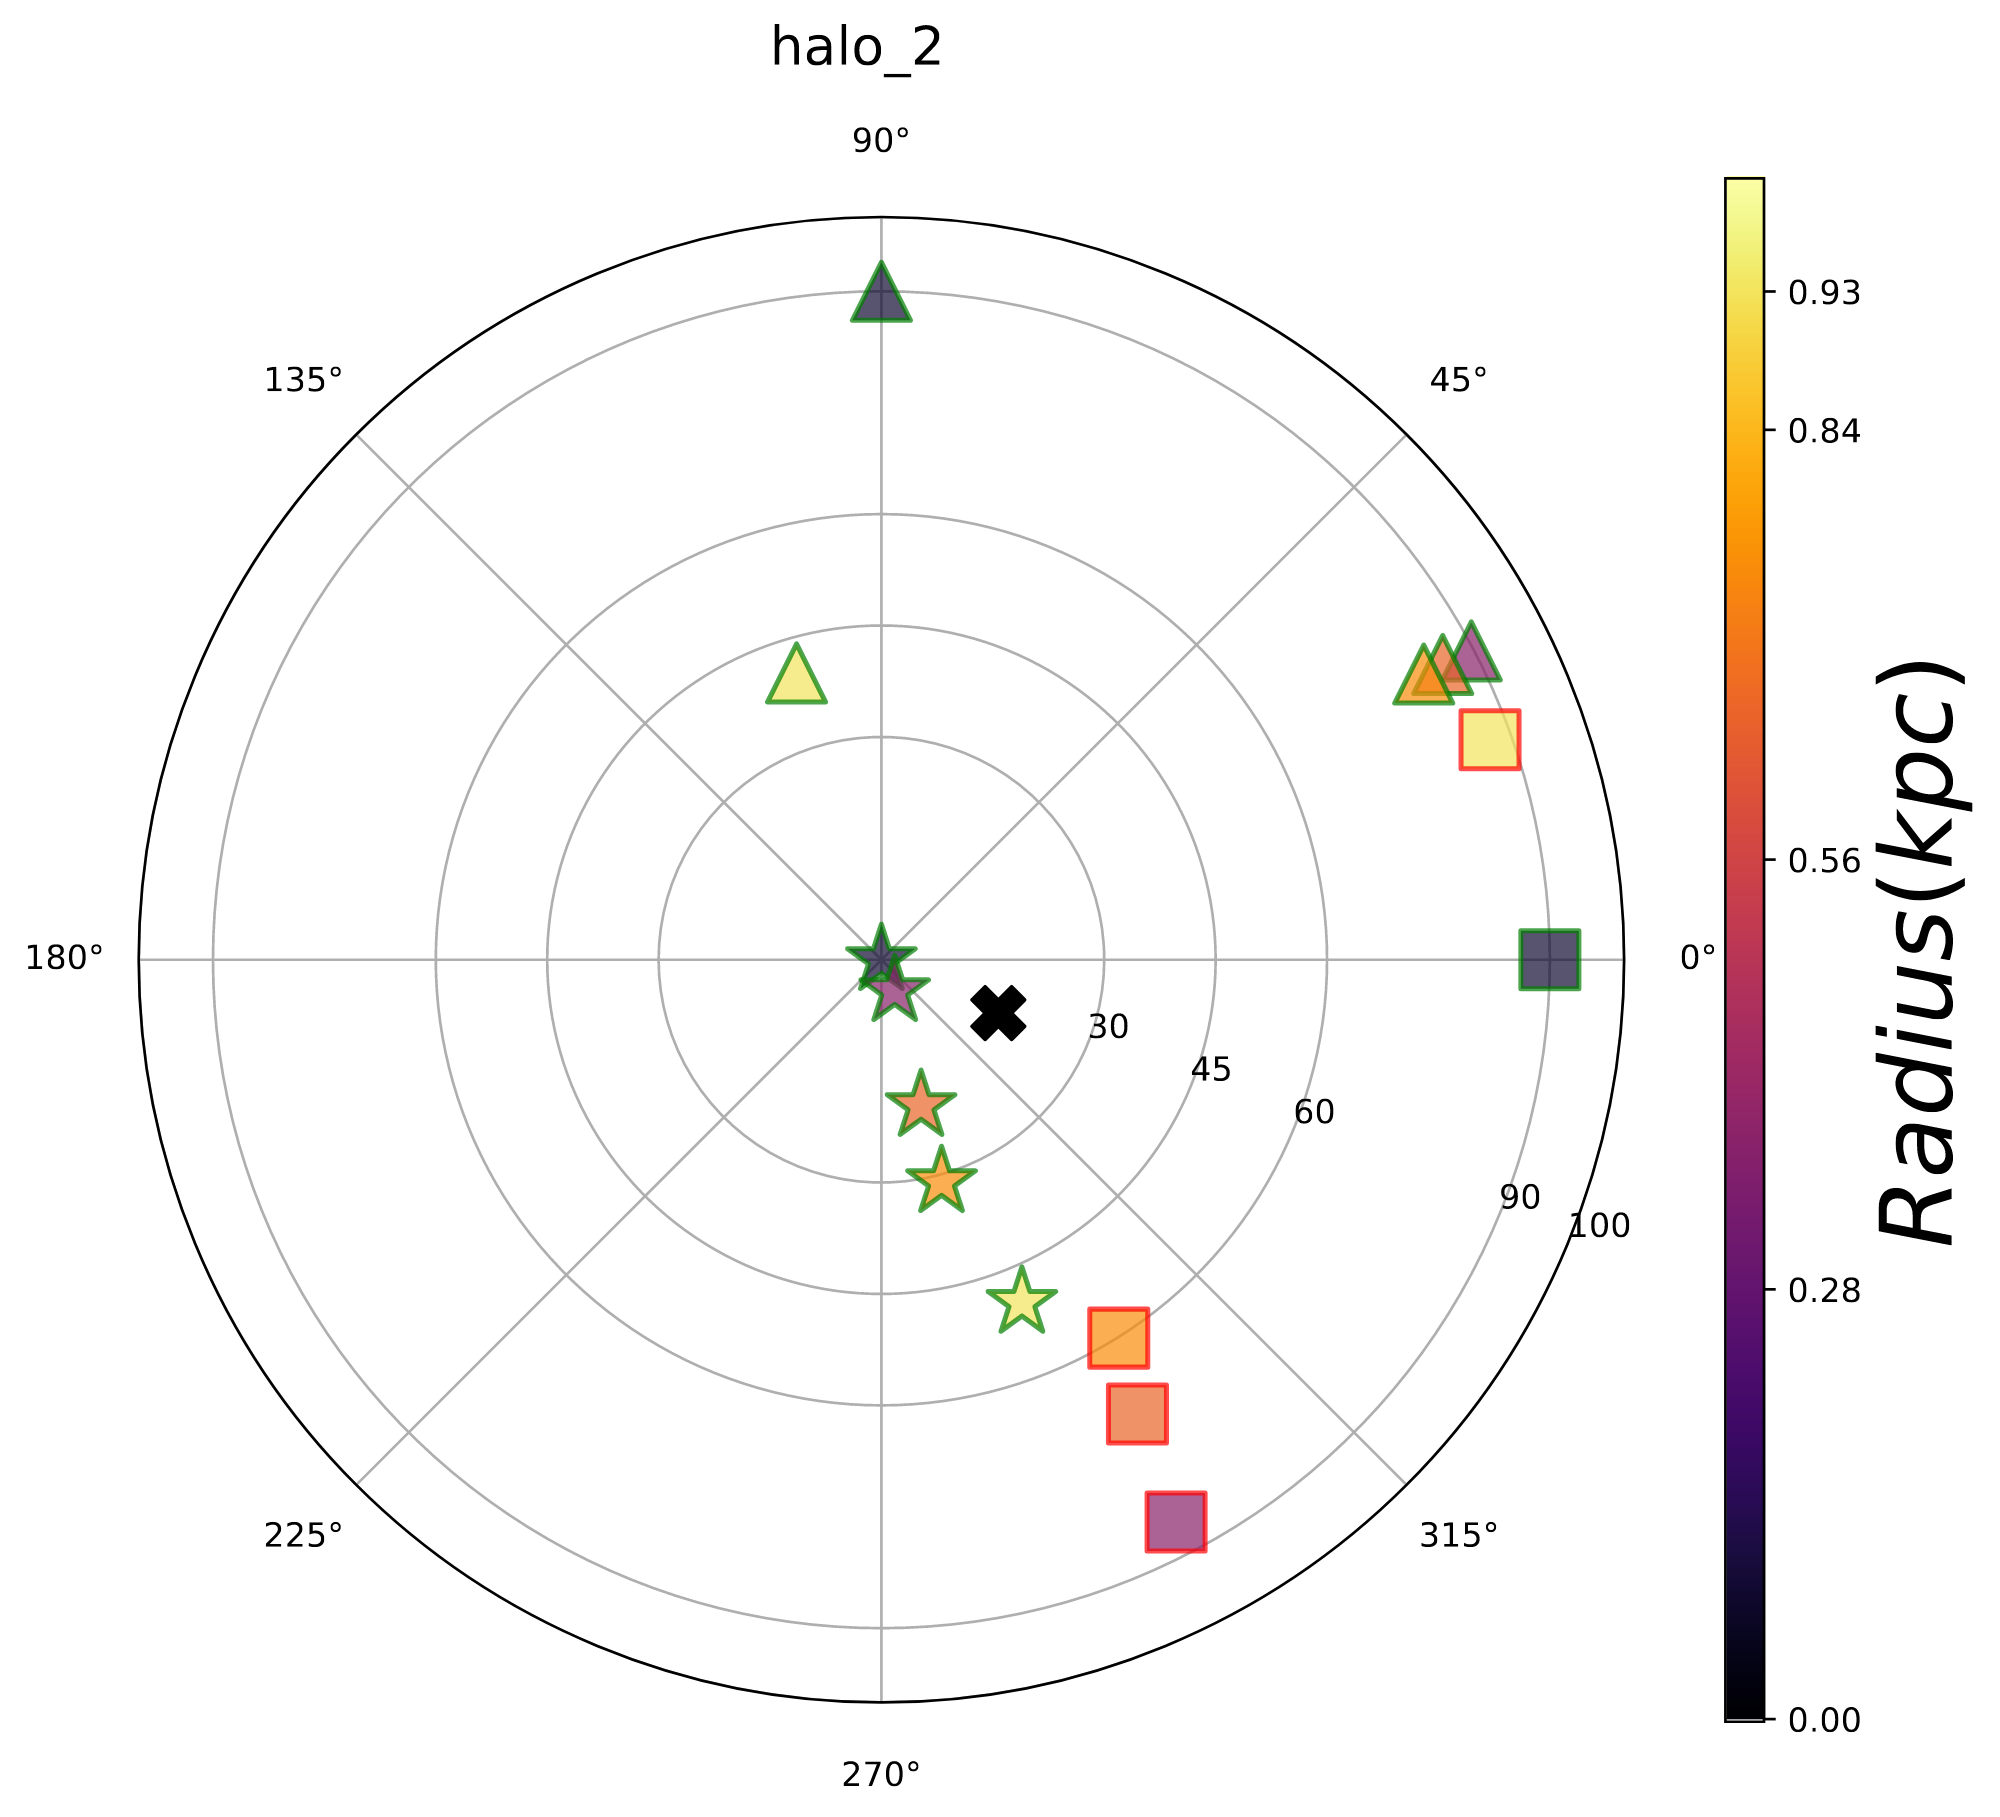
\includegraphics[width=1\columnwidth]{./pics/chaotic_axes.png}}
  \hfill
  \caption{Description of axes alignments }
  \label{fig:alignment}
\end{figure}

\textbf{Discussion about the distribution of alignments and their evolution in time: Precesion or temporary instabilities?}

\section{Conclusions}

\section{Discussion}

\section*{Acknowledgements}
This project has received funding from the European Union’s Horizon 2020 Research and Innovation Programme under the Marie Sk\l{}odowska-Curie grant agreement No 734374


%%%%%%%%%%%%%%%%%%%%%%%%%%%%%%%%%%%%%%%%%%%%%%%%%%

%%%%%%%%%%%%%%%%%%%% REFERENCES %%%%%%%%%%%%%%%%%%

% The best way to enter references is to use BibTeX:



% Alternatively you could enter them by hand, like this:
% This method is tedious and prone to error if you have lots of references
\begin{thebibliography}{99}
\bibitem[\protect\citeauthoryear{Author}{2012}]{Author2012}
Author A.~N., 2013, Journal of Improbable Astronomy, 1, 1
\bibitem[\protect\citeauthoryear{Others}{2013}]{Others2013}
Others S., 2012, Journal of Interesting Stuff, 17, 198
\end{thebibliography}

%%%%%%%%%%%%%%%%%%%%%%%%%%%%%%%%%%%%%%%%%%%%%%%%%%

%%%%%%%%%%%%%%%%% APPENDICES %%%%%%%%%%%%%%%%%%%%%

\appendix

\section{Some extra material}

If you want to present additional material which would interrupt the flow of the main paper,
it can be placed in an Appendix which appears after the list of references.

%%%%%%%%%%%%%%%%%%%%%%%%%%%%%%%%%%%%%%%%%%%%%%%%%%


% Don't change these lines
\bsp	% typesetting comment
\label{lastpage}
\end{document}

% End of mnras_template.tex
